\documentclass[a4paper,12pt]{report}
\usepackage{fancyhdr,graphicx,mathtools,multicol,titlesec,xcolor}
\usepackage{booktabs,array,caption}
\usepackage[section]{placeins}
\usepackage[top=1in, bottom=1in, left = 2cm, right = 2cm]{geometry}
\usepackage[sfdefault]{overlock}
\usepackage{hyperref}
\hypersetup{
	colorlinks=true,
	linkcolor=blue,
	filecolor=magenta,
	urlcolor=red,
	citecolor=purple,
}
\titleformat{\chapter}{\bfseries\huge}{ Chapter \thechapter. }{2pt}{}

\pagestyle{fancy}
\fancyhf{}
\rhead{IT 462 EDA }
\lhead{\includegraphics[scale=0.02]{"dau-logo.jpg"}}
\chead{\sffamily \leftmark}
\rfoot{\thepage}
\lfoot{}
\allowdisplaybreaks
\setlength{\headheight}{15pt}

% Figures live in ../figures (repository layout); a figures/ folder next to
% this file also works, e.g. when the report folder is uploaded on its own.
\graphicspath{{../figures/}{figures/}}

% Every number in this report comes from report/stats/stats.tex, generated by
% report/build_stats.py from the JSON files the notebooks write. Never type a
% statistic by hand; rerun the notebooks and build_stats.py instead.
% AUTO-GENERATED by report/build_stats.py from report/stats/*.json -- do not edit.

% ---- ch01_audit.json
% primary_rows
\newcommand{\AuditPrimaryRows}{10{,}000}
% primary_cols
\newcommand{\AuditPrimaryCols}{17}
% primary_null_release_date
\newcommand{\AuditPrimaryNullReleaseDate}{3}
% primary_null_genres
\newcommand{\AuditPrimaryNullGenres}{2}
% primary_null_production_company
\newcommand{\AuditPrimaryNullProductionCompany}{27}
% primary_null_production_country
\newcommand{\AuditPrimaryNullProductionCountry}{9}
% zero_budget
\newcommand{\AuditZeroBudget}{2{,}814}
% zero_revenue
\newcommand{\AuditZeroRevenue}{2{,}288}
% both_financials_positive
\newcommand{\AuditBothFinancialsPositive}{6{,}632}
% budget_but_zero_revenue
\newcommand{\AuditBudgetButZeroRevenue}{554}
% mean_budget_with_zeros
\newcommand{\AuditMeanBudgetWithZeros}{24{,}605{,}346}
\newcommand{\AuditMeanBudgetWithZerosM}{24.6}
% mean_budget_positive_only
\newcommand{\AuditMeanBudgetPositiveOnly}{34{,}240{,}671}
\newcommand{\AuditMeanBudgetPositiveOnlyM}{34.2}
% budget_1_to_999
\newcommand{\AuditBudgetOneToNineNineNine}{13}
% revenue_1_to_999
\newcommand{\AuditRevenueOneToNineNineNine}{9}
% zero_runtime
\newcommand{\AuditZeroRuntime}{1}
% runtime_max
\newcommand{\AuditRuntimeMax}{367}
% runtime_median
\newcommand{\AuditRuntimeMedian}{104}
% future_films
\newcommand{\AuditFutureFilms}{92}
% year_min
\newcommand{\AuditYearMin}{1895}
% year_max
\newcommand{\AuditYearMax}{2026}
% exact_duplicate_rows
\newcommand{\AuditExactDuplicateRows}{4}
% duplicated_titles
\newcommand{\AuditDuplicatedTitles}{394}
% duplicated_title_year
\newcommand{\AuditDuplicatedTitleYear}{12}
% content_rating_unrated
\newcommand{\AuditContentRatingUnrated}{1{,}165}
% content_rating_nr
\newcommand{\AuditContentRatingNr}{694}
% content_rating_stray_pg13
\newcommand{\AuditContentRatingStrayPgOneThree}{1}
% n_english
\newcommand{\AuditNEnglish}{7{,}993}
% n_languages
\newcommand{\AuditNLanguages}{44}
% total_votes_min
\newcommand{\AuditTotalVotesMin}{367}
% audience_rating_min
\newcommand{\AuditAudienceRatingMin}{2.2}
% audience_rating_max
\newcommand{\AuditAudienceRatingMax}{9.152}
% audience_rating_median
\newcommand{\AuditAudienceRatingMedian}{6.7}
% secondary_rows
\newcommand{\AuditSecondaryRows}{10{,}000}
% secondary_cols
\newcommand{\AuditSecondaryCols}{9}
% title_overlap_exact
\newcommand{\AuditTitleOverlapExact}{8{,}276}
% title_overlap_normalised
\newcommand{\AuditTitleOverlapNormalised}{8{,}307}

% ---- ch02_cleaning.json
% rows_in
\newcommand{\CleanRowsIn}{10{,}000}
% zero_budget_converted
\newcommand{\CleanZeroBudgetConverted}{2{,}814}
% zero_revenue_converted
\newcommand{\CleanZeroRevenueConverted}{2{,}288}
% budget_floored
\newcommand{\CleanBudgetFloored}{13}
% revenue_floored
\newcommand{\CleanRevenueFloored}{9}
% runtime_zeroed
\newcommand{\CleanRuntimeZeroed}{1}
% director_placeholder
\newcommand{\CleanDirectorPlaceholder}{1}
% exact_duplicates_dropped
\newcommand{\CleanExactDuplicatesDropped}{4}
% rows_after_dedupe
\newcommand{\CleanRowsAfterDedupe}{9{,}996}
% content_rating_ws_fixed
\newcommand{\CleanContentRatingWsFixed}{1}
% content_rating_nr_merged
\newcommand{\CleanContentRatingNrMerged}{692}
% country_rows_renamed
\newcommand{\CleanCountryRowsRenamed}{6{,}901}
% future_flagged
\newcommand{\CleanFutureFlagged}{92}
% has_financials
\newcommand{\CleanHasFinancials}{6{,}619}
% mar_n_doc
\newcommand{\CleanMarNDoc}{6{,}560}
% mar_n_undoc
\newcommand{\CleanMarNUndoc}{3{,}344}
% mar_p_year
\newcommand{\CleanMarPYear}{\ensuremath{6.8\times10^{-90}}}
% mar_p_votes
\newcommand{\CleanMarPVotes}{\ensuremath{<10^{-300}}}
% mar_median_votes_doc
\newcommand{\CleanMarMedianVotesDoc}{1{,}494}
% mar_median_votes_undoc
\newcommand{\CleanMarMedianVotesUndoc}{608}
% mar_median_year_doc
\newcommand{\CleanMarMedianYearDoc}{2007}
% mar_median_year_undoc
\newcommand{\CleanMarMedianYearUndoc}{2015}
% mar_median_pop_doc
\newcommand{\CleanMarMedianPopDoc}{7.5198}
% mar_median_pop_undoc
\newcommand{\CleanMarMedianPopUndoc}{4.741}
% mar_median_rating_doc
\newcommand{\CleanMarMedianRatingDoc}{6.6955}
% mar_median_rating_undoc
\newcommand{\CleanMarMedianRatingUndoc}{6.7}
% mar_p_rating
\newcommand{\CleanMarPRating}{0.102}
% mar_p_language
\newcommand{\CleanMarPLanguage}{\ensuremath{2.7\times10^{-193}}}
% mar_pct_english_doc
\newcommand{\CleanMarPctEnglishDoc}{88.3}
% mar_pct_english_undoc
\newcommand{\CleanMarPctEnglishUndoc}{63}
% secondary_matched
\newcommand{\CleanSecondaryMatched}{8{,}417}
% genres_filled
\newcommand{\CleanGenresFilled}{0}
% overviews_filled
\newcommand{\CleanOverviewsFilled}{0}
% crossval_n
\newcommand{\CleanCrossvalN}{8{,}417}
% crossval_rating_pearson
\newcommand{\CleanCrossvalRatingPearson}{0.9919}
% crossval_rating_spearman
\newcommand{\CleanCrossvalRatingSpearman}{0.9917}
% crossval_popularity_spearman
\newcommand{\CleanCrossvalPopularitySpearman}{0.7025}
% pre_1913_films
\newcommand{\CleanPreOneNineOneThreeFilms}{4}
% deflation_lost_budget_values
\newcommand{\CleanDeflationLostBudgetValues}{64}
% deflation_lost_usable
\newcommand{\CleanDeflationLostUsable}{0}
% deflate_jaws_nominal_m
\newcommand{\CleanDeflateJawsNominalM}{7.0}
% deflate_jaws_2025_m
\newcommand{\CleanDeflateJawsTwoZeroTwoFiveM}{41.9}
% deflate_titanic_nominal_m
\newcommand{\CleanDeflateTitanicNominalM}{200}
% deflate_titanic_2025_m
\newcommand{\CleanDeflateTitanicTwoZeroTwoFiveM}{401.1}
% deflate_oppenheimer_nominal_m
\newcommand{\CleanDeflateOppenheimerNominalM}{100}
% deflate_oppenheimer_2025_m
\newcommand{\CleanDeflateOppenheimerTwoZeroTwoFiveM}{105.7}
% cpi_base_year
\newcommand{\CleanCpiBaseYear}{2025}
% rows_out
\newcommand{\CleanRowsOut}{9{,}996}
% usable_financial_sample
\newcommand{\CleanUsableFinancialSample}{6{,}560}

% ---- ch03_univariate.json
% n_all
\newcommand{\UniNAll}{9{,}996}
% n_financial
\newcommand{\UniNFinancial}{6{,}560}
% budget_skew
\newcommand{\UniBudgetSkew}{2.98}
% revenue_skew
\newcommand{\UniRevenueSkew}{4.84}
% budget_median
\newcommand{\UniBudgetMedian}{20{,}000{,}000}
\newcommand{\UniBudgetMedianM}{20.0}
% revenue_median
\newcommand{\UniRevenueMedian}{39{,}197{,}782}
\newcommand{\UniRevenueMedianM}{39.2}
% runtime_skew
\newcommand{\UniRuntimeSkew}{0.25}
% rating_skew
\newcommand{\UniRatingSkew}{\ensuremath{-0.33}}
% rating_mean
\newcommand{\UniRatingMean}{6.66}
% pct_films_since_1990
\newcommand{\UniPctFilmsSinceOneNineNineZero}{84.8}
% pct_fin_since_1990
\newcommand{\UniPctFinSinceOneNineNineZero}{84.3}
% n_genres
\newcommand{\UniNGenres}{19}
% top_genre
\newcommand{\UniTopGenre}{Drama}
% top_genre_count
\newcommand{\UniTopGenreCount}{4{,}376}
% second_language
\newcommand{\UniSecondLanguage}{fr}
% second_language_count
\newcommand{\UniSecondLanguageCount}{608}
% english_to_second_ratio
\newcommand{\UniEnglishToSecondRatio}{13.1}
% n_genre_combinations_raw
\newcommand{\UniNGenreCombinationsRaw}{2{,}101}
% top_content_rating
\newcommand{\UniTopContentRating}{R}
% top_content_rating_count
\newcommand{\UniTopContentRatingCount}{4{,}015}
% runtime_median
\newcommand{\UniRuntimeMedian}{104}

% ---- ch03_multivariate.json
% n_financial
\newcommand{\MultiNFinancial}{6{,}560}
% budget_revenue_pearson_loglog
\newcommand{\MultiBudgetRevenuePearsonLoglog}{0.638}
% budget_revenue_pearson_p
\newcommand{\MultiBudgetRevenuePearsonP}{\ensuremath{<10^{-300}}}
% budget_revenue_spearman
\newcommand{\MultiBudgetRevenueSpearman}{0.675}
% pct_below_breakeven
\newcommand{\MultiPctBelowBreakeven}{26.5}
% pct_budgets_round_million
\newcommand{\MultiPctBudgetsRoundMillion}{78.7}
% flop_title_a
\newcommand{\MultiFlopTitleA}{Red Notice (2021)}
% flop_revenue_a
\newcommand{\MultiFlopRevenueA}{178{,}143}
% flop_budget_a
\newcommand{\MultiFlopBudgetA}{160{,}000{,}000}
\newcommand{\MultiFlopBudgetAM}{160.0}
% flop_title_b
\newcommand{\MultiFlopTitleB}{The Killer (2023)}
% flop_revenue_b
\newcommand{\MultiFlopRevenueB}{362{,}113}
% flop_budget_b
\newcommand{\MultiFlopBudgetB}{175{,}000{,}000}
\newcommand{\MultiFlopBudgetBM}{175.0}
% top_title_a
\newcommand{\MultiTopTitleA}{Avatar (2009)}
% top_title_b
\newcommand{\MultiTopTitleB}{Avengers: Endgame (2019)}
% genre_top_median_roi
\newcommand{\MultiGenreTopMedianRoi}{Animation}
% genre_top_median_roi_value
\newcommand{\MultiGenreTopMedianRoiValue}{2.83}
% genre_bottom_median_roi
\newcommand{\MultiGenreBottomMedianRoi}{History}
% genre_min_n
\newcommand{\MultiGenreMinN}{100}
% horror_mean_roi
\newcommand{\MultiHorrorMeanRoi}{26.39}
% horror_median_roi
\newcommand{\MultiHorrorMedianRoi}{2.43}
% animation_median_budget_m
\newcommand{\MultiAnimationMedianBudgetM}{77}
% horror_median_budget_m
\newcommand{\MultiHorrorMedianBudgetM}{15.4}
% mystery_mean_roi
\newcommand{\MultiMysteryMeanRoi}{32.69}
% mystery_median_roi
\newcommand{\MultiMysteryMedianRoi}{2.03}
% history_median_roi
\newcommand{\MultiHistoryMedianRoi}{1.53}
% rating_revenue_spearman
\newcommand{\MultiRatingRevenueSpearman}{0.074}
% rating_revenue_p
\newcommand{\MultiRatingRevenueP}{\ensuremath{2.1\times10^{-9}}}
% month_kruskal_p
\newcommand{\MultiMonthKruskalP}{\ensuremath{1.0\times10^{-44}}}
% best_month
\newcommand{\MultiBestMonth}{6}
\newcommand{\MultiBestMonthName}{June}
% best_month_median
\newcommand{\MultiBestMonthMedian}{65{,}370{,}010}
\newcommand{\MultiBestMonthMedianM}{65.4}
% worst_month
\newcommand{\MultiWorstMonth}{9}
\newcommand{\MultiWorstMonthName}{September}
% worst_month_median
\newcommand{\MultiWorstMonthMedian}{22{,}522{,}934}
\newcommand{\MultiWorstMonthMedianM}{22.5}
% n_month
\newcommand{\MultiNMonth}{6{,}560}
% july_median
\newcommand{\MultiJulyMedian}{59{,}999{,}667}
\newcommand{\MultiJulyMedianM}{60.0}
% december_median
\newcommand{\MultiDecemberMedian}{58{,}469{,}210}
\newcommand{\MultiDecemberMedianM}{58.5}
% june_to_september_ratio
\newcommand{\MultiJuneToSeptemberRatio}{2.9}
% roi_budget_spearman
\newcommand{\MultiRoiBudgetSpearman}{\ensuremath{-0.13}}
% votes_revenue_spearman
\newcommand{\MultiVotesRevenueSpearman}{0.656}
% rating_votes_spearman
\newcommand{\MultiRatingVotesSpearman}{0.306}
% budget_year_spearman
\newcommand{\MultiBudgetYearSpearman}{0}
% roi_budget_spearman_p
\newcommand{\MultiRoiBudgetSpearmanP}{\ensuremath{4.6\times10^{-26}}}
% runtime_rating_spearman
\newcommand{\MultiRuntimeRatingSpearman}{0.292}
% runtime_rating_p
\newcommand{\MultiRuntimeRatingP}{\ensuremath{2.5\times10^{-196}}}
% runtime_rating_n
\newcommand{\MultiRuntimeRatingN}{9{,}995}
% decade_1970_median_budget_m
\newcommand{\MultiDecadeOneNineSevenZeroMedianBudgetM}{20.9}
% decade_1970_median_roi
\newcommand{\MultiDecadeOneNineSevenZeroMedianRoi}{6.25}
% decade_1970_n
\newcommand{\MultiDecadeOneNineSevenZeroN}{217}
% decade_1990_median_budget_m
\newcommand{\MultiDecadeOneNineNineZeroMedianBudgetM}{52.8}
% decade_1990_median_roi
\newcommand{\MultiDecadeOneNineNineZeroMedianRoi}{2.07}
% decade_1990_n
\newcommand{\MultiDecadeOneNineNineZeroN}{940}
% decade_2010_median_budget_m
\newcommand{\MultiDecadeTwoZeroOneZeroMedianBudgetM}{27.2}
% decade_2010_median_roi
\newcommand{\MultiDecadeTwoZeroOneZeroMedianRoi}{2.14}
% decade_2010_n
\newcommand{\MultiDecadeTwoZeroOneZeroN}{2{,}121}
% decade_2020_median_budget_m
\newcommand{\MultiDecadeTwoZeroTwoZeroMedianBudgetM}{27}
% decade_2020_median_roi
\newcommand{\MultiDecadeTwoZeroTwoZeroMedianRoi}{1.38}
% decade_2020_n
\newcommand{\MultiDecadeTwoZeroTwoZeroN}{738}
% value_top_genre
\newcommand{\MultiValueTopGenre}{Horror}
% value_top_ratio
\newcommand{\MultiValueTopRatio}{4.09}
% value_second_genre
\newcommand{\MultiValueSecondGenre}{Drama}
% value_bottom_genre
\newcommand{\MultiValueBottomGenre}{Adventure}
% value_bottom_ratio
\newcommand{\MultiValueBottomRatio}{0.77}
% value_top_rating_genre
\newcommand{\MultiValueTopRatingGenre}{War}
% value_top_rating
\newcommand{\MultiValueTopRating}{7.18}
% genre_budget_rating_spearman
\newcommand{\MultiGenreBudgetRatingSpearman}{0.189}
% genre_budget_rating_p
\newcommand{\MultiGenreBudgetRatingP}{0.468}
% genre_budget_rating_n
\newcommand{\MultiGenreBudgetRatingN}{17}
% mid_n
\newcommand{\MultiMidN}{1{,}893}
% mid_roi_2000s
\newcommand{\MultiMidRoiTwoZeroZeroZeros}{1.78}
% mid_roi_2010s
\newcommand{\MultiMidRoiTwoZeroOneZeros}{1.89}
% mid_roi_2020s
\newcommand{\MultiMidRoiTwoZeroTwoZeros}{1.0}
% mid_pct_prof_2000s
\newcommand{\MultiMidPctProfTwoZeroZeroZeros}{70.4}
% mid_pct_prof_2010s
\newcommand{\MultiMidPctProfTwoZeroOneZeros}{70}
% mid_pct_prof_2020s
\newcommand{\MultiMidPctProfTwoZeroTwoZeros}{50.2}
% mid_n_2000s
\newcommand{\MultiMidNTwoZeroZeroZeros}{785}
% mid_n_2010s
\newcommand{\MultiMidNTwoZeroOneZeros}{829}
% mid_n_2020s
\newcommand{\MultiMidNTwoZeroTwoZeros}{279}
% mid_kruskal_p
\newcommand{\MultiMidKruskalP}{\ensuremath{2.5\times10^{-10}}}
% mid_chi2_p
\newcommand{\MultiMidChiTwoP}{\ensuremath{3.9\times10^{-10}}}
% mid_2000s_vs_2010s_p
\newcommand{\MultiMidTwoZeroZeroZerosVsTwoZeroOneZerosP}{0.879}

% ---- ch04_features.json
% n_financial
\newcommand{\FeatNFinancial}{6{,}560}
% pct_profitable
\newcommand{\FeatPctProfitable}{73.4}
% director_check_matched
\newcommand{\FeatDirectorCheckMatched}{500}
% director_check_n
\newcommand{\FeatDirectorCheckN}{500}
% n_engineered
\newcommand{\FeatNEngineered}{33}
% studio_tier_major
\newcommand{\FeatStudioTierMajor}{2{,}054}
% studio_tier_mid
\newcommand{\FeatStudioTierMid}{3{,}057}
% studio_tier_indie
\newcommand{\FeatStudioTierIndie}{4{,}858}
% tier_major_median_revenue_m
\newcommand{\FeatTierMajorMedianRevenueM}{83.4}
% tier_mid_median_revenue_m
\newcommand{\FeatTierMidMedianRevenueM}{46.8}
% tier_indie_median_revenue_m
\newcommand{\FeatTierIndieMedianRevenueM}{16.9}
% n_summer
\newcommand{\FeatNSummer}{2{,}288}
% n_holiday
\newcommand{\FeatNHoliday}{1{,}861}
% collinear_pairs_over_0p8
\newcommand{\FeatCollinearPairsOverZeropEight}{0}
% max_vif
\newcommand{\FeatMaxVif}{1.33}
% genre_count_equals_flag_sum
\newcommand{\FeatGenreCountEqualsFlagSum}{yes}
% mi_top_revenue_feature
\newcommand{\FeatMiTopRevenueFeature}{log\_budget\_2025}
% mi_budget_revenue
\newcommand{\FeatMiBudgetRevenue}{0.347}
% mi_budget_roi
\newcommand{\FeatMiBudgetRoi}{0.068}
% mi_votes_revenue_leaky
\newcommand{\FeatMiVotesRevenueLeaky}{0.357}
% mi_votes_roi_leaky
\newcommand{\FeatMiVotesRoiLeaky}{0.107}
% mi_votes_profitable_leaky
\newcommand{\FeatMiVotesProfitableLeaky}{0.08}
% mi_best_legit_profitable
\newcommand{\FeatMiBestLegitProfitable}{0.009}
% mi_leak_ratio_profitable
\newcommand{\FeatMiLeakRatioProfitable}{8.8}
% mi_roi_to_revenue_ratio_budget
\newcommand{\FeatMiRoiToRevenueRatioBudget}{0.2}

% ---- ch05_modelling.json
% n_model
\newcommand{\ModelNModel}{6{,}560}
% split_year
\newcommand{\ModelSplitYear}{2017}
% n_train
\newcommand{\ModelNTrain}{5{,}431}
% n_test
\newcommand{\ModelNTest}{1{,}129}
% ols_dropped_degenerate
\newcommand{\ModelOlsDroppedDegenerate}{genre\_tv\_movie}
% ols_rev_r2_train
\newcommand{\ModelOlsRevRTwoTrain}{0.456}
% ols_rev_r2_test
\newcommand{\ModelOlsRevRTwoTest}{0.361}
% ols_bp_p
\newcommand{\ModelOlsBpP}{\ensuremath{3.9\times10^{-75}}}
% ols_coef_tier_major
\newcommand{\ModelOlsCoefTierMajor}{0.692}
% ols_p_tier_major
\newcommand{\ModelOlsPTierMajor}{\ensuremath{5.1\times10^{-46}}}
% ols_coef_tier_mid
\newcommand{\ModelOlsCoefTierMid}{0.36}
% ols_p_tier_mid
\newcommand{\ModelOlsPTierMid}{\ensuremath{7.2\times10^{-12}}}
% ols_coef_is_holiday_release
\newcommand{\ModelOlsCoefIsHolidayRelease}{0.234}
% ols_p_is_holiday_release
\newcommand{\ModelOlsPIsHolidayRelease}{\ensuremath{2.1\times10^{-6}}}
% ols_coef_is_summer_release
\newcommand{\ModelOlsCoefIsSummerRelease}{0.198}
% ols_p_is_summer_release
\newcommand{\ModelOlsPIsSummerRelease}{\ensuremath{3.4\times10^{-5}}}
% ols_coef_is_english
\newcommand{\ModelOlsCoefIsEnglish}{0.224}
% ols_p_is_english
\newcommand{\ModelOlsPIsEnglish}{0.006}
% ols_coef_genre_documentary
\newcommand{\ModelOlsCoefGenreDocumentary}{0.871}
% ols_p_genre_documentary
\newcommand{\ModelOlsPGenreDocumentary}{0.001}
% ols_coef_genre_animation
\newcommand{\ModelOlsCoefGenreAnimation}{0.329}
% ols_p_genre_animation
\newcommand{\ModelOlsPGenreAnimation}{\ensuremath{2.7\times10^{-4}}}
% ols_coef_genre_horror
\newcommand{\ModelOlsCoefGenreHorror}{\ensuremath{-0.108}}
% ols_p_genre_horror
\newcommand{\ModelOlsPGenreHorror}{0.182}
% ols_coef_director_mean_prior_rating
\newcommand{\ModelOlsCoefDirectorMeanPriorRating}{0.128}
% ols_p_director_mean_prior_rating
\newcommand{\ModelOlsPDirectorMeanPriorRating}{0.005}
% ols_coef_runtime_mins
\newcommand{\ModelOlsCoefRuntimeMins}{0.011}
% ols_p_runtime_mins
\newcommand{\ModelOlsPRuntimeMins}{\ensuremath{4.5\times10^{-16}}}
% ols_budget_elasticity
\newcommand{\ModelOlsBudgetElasticity}{0.698}
% ols_budget_p
\newcommand{\ModelOlsBudgetP}{\ensuremath{3.7\times10^{-141}}}
% ols_budget_ci_lo
\newcommand{\ModelOlsBudgetCiLo}{0.644}
% ols_budget_ci_hi
\newcommand{\ModelOlsBudgetCiHi}{0.752}
% ols_resid_skew
\newcommand{\ModelOlsResidSkew}{\ensuremath{-1.03}}
% ridge_rev_r2_test
\newcommand{\ModelRidgeRevRTwoTest}{0.381}
% gb_rev_r2_test
\newcommand{\ModelGbRevRTwoTest}{0.364}
% ols_rev_rmse_test
\newcommand{\ModelOlsRevRmseTest}{1.716}
% ridge_rev_rmse_test
\newcommand{\ModelRidgeRevRmseTest}{1.689}
% ols_roi_r2_test
\newcommand{\ModelOlsRoiRTwoTest}{0.031}
% gb_roi_r2_test
\newcommand{\ModelGbRoiRTwoTest}{0.042}
% roi_budget_coef
\newcommand{\ModelRoiBudgetCoef}{\ensuremath{-0.302}}
% roi_budget_p
\newcommand{\ModelRoiBudgetP}{\ensuremath{6.2\times10^{-28}}}
% ridge_roi_r2_test
\newcommand{\ModelRidgeRoiRTwoTest}{0.061}
% roi_budget_ci_lo
\newcommand{\ModelRoiBudgetCiLo}{\ensuremath{-0.356}}
% roi_budget_ci_hi
\newcommand{\ModelRoiBudgetCiHi}{\ensuremath{-0.248}}
% class_balance_train
\newcommand{\ModelClassBalanceTrain}{75.4}
% class_balance_test
\newcommand{\ModelClassBalanceTest}{63.9}
% clf_best_auc
\newcommand{\ModelClfBestAuc}{0.682}
% clf_best_f1
\newcommand{\ModelClfBestFOne}{0.783}
% majority_baseline_f1
\newcommand{\ModelMajorityBaselineFOne}{0.779}
% clf_logistic_precision
\newcommand{\ModelClfLogisticPrecision}{0.647}
% clf_logistic_recall
\newcommand{\ModelClfLogisticRecall}{0.99}
% clf_logistic_auc
\newcommand{\ModelClfLogisticAuc}{0.682}
% clf_logistic_f1
\newcommand{\ModelClfLogisticFOne}{0.783}
% clf_histgb_precision
\newcommand{\ModelClfHistgbPrecision}{0.659}
% clf_histgb_recall
\newcommand{\ModelClfHistgbRecall}{0.956}
% clf_histgb_auc
\newcommand{\ModelClfHistgbAuc}{0.643}
% clf_histgb_f1
\newcommand{\ModelClfHistgbFOne}{0.78}
% perm_top_feature
\newcommand{\ModelPermTopFeature}{log\_budget\_2025}
% perm_top_drop
\newcommand{\ModelPermTopDrop}{0.474}
% perm_second_drop
\newcommand{\ModelPermSecondDrop}{0.058}
% perm_second_feature
\newcommand{\ModelPermSecondFeature}{studio\_tier}


\captionsetup{font=small, labelfont=bf}
\newcommand{\code}[1]{\texttt{#1}}
\newcommand{\tablein}[1]{\input{tables/#1.tex}}

% ---- details still to be filled in by the group (shown in red until then)
\newcommand{\groupno}{\textcolor{red}{[group no.]}}

% Define a macro to create the parboxes for each member
\newcommand{\member}[4]{
    \parbox{.22\linewidth}{\centering
        \includegraphics[width=2cm]{#1} \\  % #1 for image path
        \par #2 \\                          % #2 for name
        \emph{ID:} #3 \\                    % #3 for ID
        \emph{Course:} #4                   % #4 for course
    }
}
\newcommand{\projecttitle}[1]{
    \vspace{.1\textheight}
    {\textbf{\Huge Exploratory Data Analysis\\ on} \par}
    \vspace{.3cm}
    {\Large \scshape #1 \par} % Custom title from the argument
    \vspace{.5cm}
}
\begin{document}
\begin{titlepage}
\centering
	\projecttitle{Understanding What Makes a Movie Successful}
		by \par
{ \Huge Group \groupno \par }

\vspace{0.5cm}

% Signature images: replace dau-logo.jpg with each member's signature scan.
    \member{dau-logo.jpg}{Kirtan Kamani}{202401094}{BTech} \hfil
    \member{dau-logo.jpg}{Khanjan Shah}{202401092}{BTech} \hfil
    \member{dau-logo.jpg}{Shyam Bhuva}{202401034}{BTech}\hfil
    \member{dau-logo.jpg}{Het Bhungaliya}{202401033}{BTech}

\vspace{1cm}

{ \Large Course Code: IT 462 \par

Semester: Autumn 2026 \par }

\rule{.3\textwidth}{.1pt}\par
\vspace{.2cm}
		Under the guidance of \par
	\vspace{.2cm}
		{\Large\bfseries Dr. Gopinath Panda\par}

		\vfill

		\includegraphics[scale=0.25]{"dau-logo.jpg"}

		{\large \today\par}
	\end{titlepage}
\newpage
\begin{center}
\textsc{\huge Acknowledgment}
\end{center}
\thispagestyle{empty}
	\bigskip

We are grateful to Dr.\ Gopinath Panda for his guidance throughout IT 462 and this project. The course's insistence on looking hard at data before modelling it shaped every chapter of this report, from the decision not to impute missing budgets to the habit of reporting a sample size beside every statistic.

We thank Dhirubhai Ambani University for the facilities and the academic environment that made this work possible.

The data behind this project comes from The Movie Database (TMDB). This product uses the TMDB API but is not endorsed or certified by TMDB. We also thank the author of the Kaggle collection \emph{Top Rated TMDB Movies 10K}, which we used to cross-validate our scraped data, and the Federal Reserve Bank of St.\ Louis, whose FRED service provides the consumer price index we used to adjust for inflation.

Finally, we thank our classmates for discussions that sharpened several of the questions asked here.

\vspace{2cm}
	Sincerely,

	Kirtan Kamani (202401094), Khanjan Shah (202401092), Shyam Bhuva (202401034), Het Bhungaliya (202401033)



\newpage

\begin{center}
	\textbf{\huge DECLARATION}
\end{center}
\thispagestyle{empty}
\vspace{2cm}

We, Kirtan Kamani, Khanjan Shah, Shyam Bhuva and Het Bhungaliya, hereby declare that the EDA project work presented in this report is our original work and has not been submitted for any other academic degree. All the sources cited in this report have been appropriately referenced.

We acknowledge that the primary dataset used in this project was collected from The Movie Database (\url{https://www.themoviedb.org}) through its public API, and that the secondary dataset was obtained from Kaggle (\emph{Top Rated TMDB Movies 10K}). We declare that we have adhered to the terms and conditions of both sources for using the data. We confirm that the datasets used in this project are true and accurate to the best of our knowledge, and that every known defect in them is documented in Chapter~\ref{ch:cleaning}.

We acknowledge that we have received no external help or assistance in conducting this project, except for the guidance provided by our mentor Dr.\ Gopinath Panda. We declare that there is no conflict of interest in conducting this EDA project.

We hereby sign the declaration statement and confirm the submission of this report on \today.

\vspace{2cm}

% Replace dau-logo.jpg with each member's signature scan.
    \member{dau-logo.jpg}{Kirtan Kamani}{202401094}{BTech} \hfil
    \member{dau-logo.jpg}{Khanjan Shah}{202401092}{BTech} \hfil
    \member{dau-logo.jpg}{Shyam Bhuva}{202401034}{BTech} \hfil
    \member{dau-logo.jpg}{Het Bhungaliya}{202401033}{BTech}

\newpage
\begin{center}
	\textbf{\huge \scshape CERTIFICATE}
\end{center}
\thispagestyle{empty}
\vspace{2cm}

This is to certify that Group \groupno{} comprising Kirtan Kamani (202401094), Khanjan Shah (202401092), Shyam Bhuva (202401034) and Het Bhungaliya (202401033) has successfully completed an exploratory data analysis (EDA) project on \emph{Understanding What Makes a Movie Successful}, using film data collected from The Movie Database (TMDB) through its public API, together with a secondary TMDB-derived collection from Kaggle.

The EDA project presented by Group \groupno{} is their original work and has been completed under the guidance of the course instructor, Dr.\ Gopinath Panda, who has provided support and guidance throughout the project. The project is based on a thorough analysis of the TMDB datasets, and the results presented in the report are based on the data obtained from those datasets.

This certificate is issued to recognize the successful completion of the EDA project on \emph{Understanding What Makes a Movie Successful}, which demonstrates the analytical skills and knowledge of the students of Group \groupno{} in the field of data analysis.


\vfill
Signed,\par
Dr. Gopinath Panda,\par
IT 462 Course Instructor\par
Dhirubhai Ambani University\par
Gandhinagar, Gujarat, INDIA.\par

\today

%%%%%%%%%%%%%%%%%%%%%%%%%%%%%%%%%%
	\tableofcontents
\addcontentsline{toc}{chapter}{\listfigurename}
\listoffigures
\listoftables
%%%%%%%%%%%%%%%%%%%%%%%%%%%%%%%%%%
\begin{abstract}

Most films do not earn back what they cost, so it matters which attributes of a film travel with commercial and critical success. We analyse \AuditPrimaryRows{} films scraped from The Movie Database (TMDB), cross-checked against a second, independently assembled collection of \AuditSecondaryRows{} TMDB films from Kaggle.

The central data problem is that TMDB records an unknown budget or revenue as zero. Only \CleanUsableFinancialSample{} released films have both figures. Films without them differ sharply from films with them: they have far fewer votes, are less popular, are less often in English and are \emph{newer}. Their ratings, however, are no different. We therefore analyse the documented films as they are and do not impute missing money, which restricts our financial conclusions to well-documented, mostly mainstream cinema. All money is converted to constant \CleanCpiBaseYear{} dollars.

Budget is strongly associated with gross revenue: a 1\% larger budget goes with about \ModelOlsBudgetElasticity\% more gross. But budget is \emph{negatively} associated with return on investment (Spearman $r=\MultiRoiBudgetSpearman$, $n=\MultiNFinancial$). Pre-release attributes explain about a third of the variance in log revenue on films from later years than the ones the models were trained on (test $R^2=\ModelRidgeRevRTwoTest$), but almost none of the variance in log ROI (test $R^2\le\ModelRidgeRoiRTwoTest$). The scale of a film's gross is fairly predictable from what the film is; its return per dollar is not. Audience rating is nearly unrelated to revenue ($r=\MultiRatingRevenueSpearman$). Summer and winter-holiday releases earn more, and the median ROI of mid-budget films fell sharply after 2019.

Every association reported here is observational. Marketing spend, plausibly the largest omitted variable, is absent from the data.

\end{abstract}

%%%%%%%%%%%%%%%%%%%%%%%%%%%%%%%%%%%%%%%%%%%%%%%%%%%%%%%%%%%%%%%%%%%%%%%%%%%
\chapter{Introduction}\label{ch:intro}
%%%%%%%%%%%%%%%%%%%%%%%%%%%%%%%%%%%%%%%%%%%%%%%%%%%%%%%%%%%%%%%%%%%%%%%%%%%

\section{Project idea}

The film industry invests billions of dollars every year, yet a large share of films fail to break even. This project asks which measurable attributes of a film are associated with its commercial success (worldwide revenue and return on investment) and its critical success (audience rating). The attributes considered are budget, runtime, genre, director history, production company, release timing and original language. The goal is to measure those associations carefully, and to say plainly where the data cannot support a claim about cause.

Rather than a general theme, the project answers five specific questions:

\begin{enumerate}
  \item \textbf{Does a larger budget buy a higher return, or only a higher gross?}
  \item \textbf{Which genres give the best audience rating per dollar of budget?}
  \item \textbf{Has the profitability of a mid-budget film changed since 2000?}
  \item \textbf{Is release timing associated with revenue?} In particular, do the summer and winter-holiday windows earn more?
  \item \textbf{Do critical and commercial success go together?} And how much of either can be predicted from attributes known before release?
\end{enumerate}

Chapter~\ref{ch:conclusion} answers each question directly, with numbers.

This is an exploratory analysis of observational data. Big budgets travel with big marketing campaigns, star casts and wide releases, and marketing spend is not in the data. So throughout this report we write that a variable \emph{is associated with} an outcome; no statement in it is a causal claim.

\section{Data Collection}

The project uses two files, collected in two different ways.

\paragraph{Primary dataset: scraped from the TMDB API.} \code{movies\_eda\_checkpoint\_2.csv} was assembled by querying the public API of The Movie Database (\url{https://www.themoviedb.org}) for each film's details, credits and release information, then flattening the responses into one row per film. It holds \AuditPrimaryRows{} films and \AuditPrimaryCols{} columns. It is the only file with budget and revenue, so the whole analysis rests on it. TMDB is community-edited: budgets and revenues are contributed by users and editors, not audited, and an unknown value is stored as zero (Chapter~\ref{ch:cleaning}).

\paragraph{Secondary dataset: downloaded from Kaggle.} \code{top10K-TMDB-movies.csv} is the public Kaggle collection \emph{Top Rated TMDB Movies 10K} (\code{ahsanaseer/top-rated-tmdb-movies-10k}) \cite{kaggle}. It holds \AuditSecondaryRows{} films and \AuditSecondaryCols{} columns, also drawn from TMDB, but has no budget or revenue. We use it for exactly three things:
\begin{enumerate}
  \item cross-validating ratings and popularity on the films both files share;
  \item recovering the TMDB \code{id} as a stable join key;
  \item filling missing genres and overviews in the primary file.
\end{enumerate}

\paragraph{Overlap, and why the files are not stacked.} After trimming whitespace and ignoring case, \AuditTitleOverlapNormalised{} titles appear in both files (\AuditTitleOverlapExact{} on exact string match). The two files are overlapping samples of the same population with different schemas. Concatenating them into one 20{,}000-row table would count most films twice, so we never do. Instead the secondary file is joined onto the primary one by title and release year (Section~\ref{sec:secondary}).

\paragraph{Inflation data.} To make dollars comparable across more than a century, we use the US Consumer Price Index for All Urban Consumers (FRED series \code{CPIAUCNS}) \cite{fred}, downloaded as monthly values and committed unchanged to \code{data/raw/}.

\section{Dataset Description}

Tables~\ref{tab:primary} and~\ref{tab:secondary} describe both files as stored, before any cleaning. Four columns of the primary file hold several values in one comma-separated string: \code{Genres}, \code{Lead\_Actors}, \code{Production\_Company} and \code{Production\_Country}. These are handled in Chapter~\ref{ch:features}. Release years span \AuditYearMin{}--\AuditYearMax{}. Every film has at least \AuditTotalVotesMin{} audience votes: the collection was already filtered to films that enough people rated, which matters for every conclusion (Section~\ref{sec:challenges}).

\begin{table}[htbp]
\centering\small
\tablein{tab1_1_primary_schema}
\caption{Primary dataset as stored (\AuditPrimaryRows{} rows). ``Non-null'' counts true nulls only: the zeros that stand for unknown budget and revenue look complete here, which is exactly the trap Chapter~\ref{ch:cleaning} deals with.}
\label{tab:primary}
\end{table}

\begin{table}[htbp]
\centering\small
\tablein{tab1_2_secondary_schema}
\caption{Secondary (Kaggle) dataset as stored (\AuditSecondaryRows{} rows). It carries a TMDB \code{id} but no financial columns, so it cannot support any analysis of commercial success on its own.}
\label{tab:secondary}
\end{table}

\section{Packages required}

All analysis runs in Python, in six notebooks that run top to bottom on a fresh kernel. Shared code lives in four modules under \code{src/}: \code{load.py} (readers, data types, the zero-to-missing rule), \code{clean.py} (every cleaning rule as a named function), \code{features.py} (engineered columns) and \code{plotting.py} (one plotting style for every figure). The notebooks write every statistic quoted in this report to JSON files. A script turns those files into the LaTeX macros used in the text, so no number here is typed by hand. Table~\ref{tab:packages} lists the pinned package versions.

\begin{table}[htbp]
\centering\small
\tablein{tab1_3_packages}
\caption{Pinned package versions, generated from \code{requirements.txt}.}
\label{tab:packages}
\end{table}

%%%%%%%%%%%%%%%%%%%%%%%%%%%%%%%%%%%%%%%%%%%%%%%%%%%%%%%%%%%%%%%%%%%%%%%%%%%
\chapter{Data Cleaning}\label{ch:cleaning}
%%%%%%%%%%%%%%%%%%%%%%%%%%%%%%%%%%%%%%%%%%%%%%%%%%%%%%%%%%%%%%%%%%%%%%%%%%%

This chapter handles each known defect in the primary file and explains each choice. One principle holds throughout: \textbf{no row leaves the dataset silently}. Only exact duplicate rows are dropped. Every other problem is either converted to a missing value or flagged and excluded from the analyses it would distort, and Table~\ref{tab:recon} accounts for every row.

\section{Zero-coded financials}

TMDB stores an \emph{unknown} budget or revenue as \code{0}, not as a blank. A zero budget does not mean a film cost nothing, and a zero revenue does not mean nobody watched it; both mean the field is empty. In the raw file \AuditZeroBudget{} films have a zero budget and \AuditZeroRevenue{} a zero revenue. Only \AuditBothFinancialsPositive{} have both figures above zero, and a further \AuditBudgetButZeroRevenue{} have a budget but no revenue.

Treating those zeros as real values distorts every financial statistic. The mean budget computed with the zeros included is \$\AuditMeanBudgetWithZerosM{}M; over recorded budgets only it is \$\AuditMeanBudgetPositiveOnlyM{}M. The first figure understates the second by more than a quarter. We therefore convert all zeros in both columns to missing values when the data is first loaded (Table~\ref{tab:zero}), so no later step can accidentally average them in.

\begin{table}[htbp]
\centering\small
\tablein{tab2_1_zero_conversion}
\caption{Converting zeros to missing values. Before conversion both columns look complete; afterwards the true gaps are visible.}
\label{tab:zero}
\end{table}

\section{Missing data analysis}

\subsection{Missing values by column}

With the zero coding undone, Table~\ref{tab:missing} shows the real extent of missing data. Financial data is the only serious gap: more than a quarter of budgets and almost a quarter of revenues are unknown. Every other column is over 99\% complete. Figure~\ref{fig:matrix} shows where the gaps sit.

\begin{table}[htbp]
\centering\small
\tablein{tab2_2_missing_by_column}
\caption{Missing values by column after zeros become missing values. Only the two financial columns have substantial gaps.}
\label{tab:missing}
\end{table}

\begin{figure}[htbp]
\centering
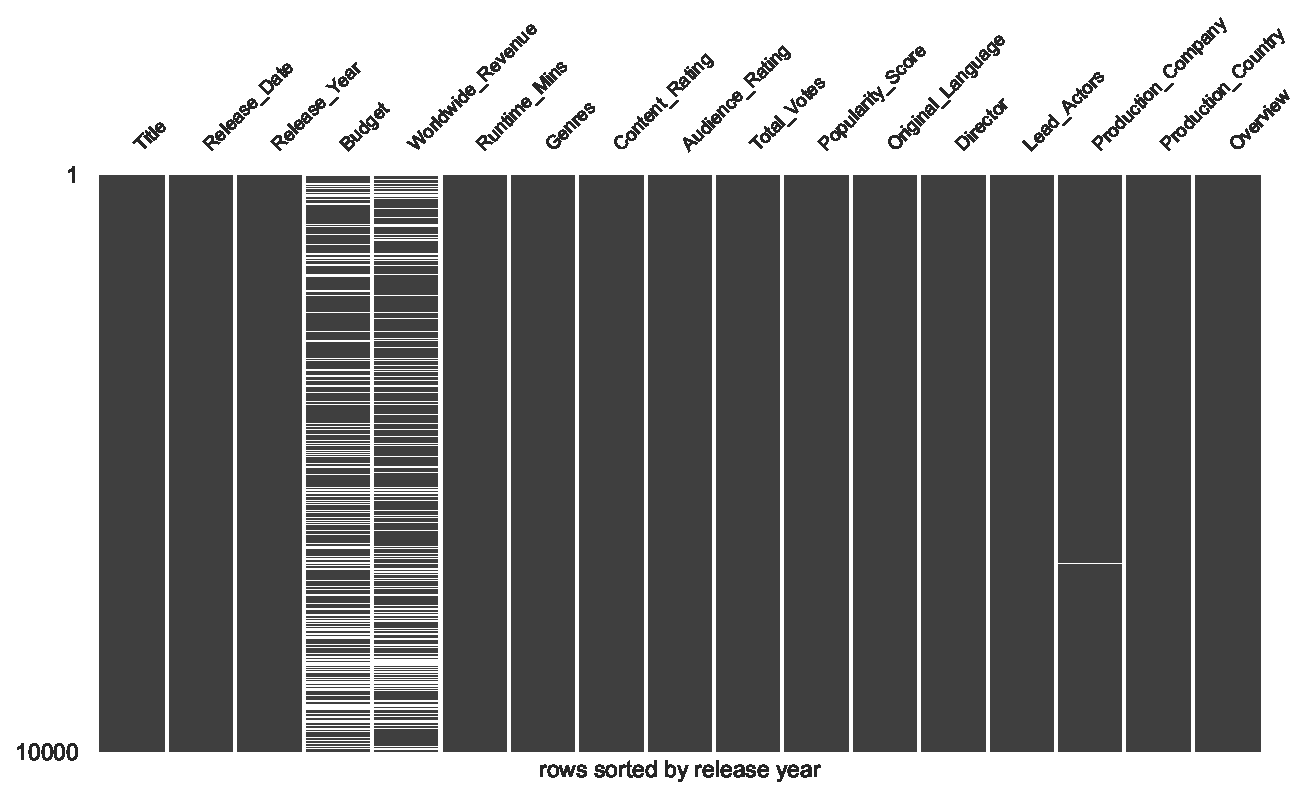
\includegraphics[width=\linewidth]{fig2_1_missing_matrix}
\caption{Missingness matrix, with rows sorted by release year from oldest (top) to newest (bottom); white marks a missing value. The gaps in \code{Budget} and \code{Worldwide\_Revenue} are not scattered evenly: they grow denser towards the bottom of the matrix, among the most recent films. That pattern was the first sign that the missingness is not random.}
\label{fig:matrix}
\end{figure}

\subsection{Is the missingness random?}

Whether missing values can be imputed depends on why they are missing \cite{rubin1976,littlerubin}. If budgets were missing \emph{completely at random} (MCAR), films with and without financials would look alike on every other variable, and filling the gaps with a median would be defensible. We tested this directly. Among released films, we compared the \CleanMarNDoc{} with both financials against the \CleanMarNUndoc{} without, on release year, vote count, audience rating, popularity and language. Films dated after 2025 are left out of this comparison, because their revenue is missing for a different reason: it does not exist yet. The numeric variables are heavily skewed, so we used the Mann--Whitney $U$ test, which does not assume normality. The effect size is the rank-biserial correlation $r = 1 - 2U/(n_1 n_2)$, where a negative value means documented films tend to have higher values. Language was tested with a chi-square test. Table~\ref{tab:mar} and Figure~\ref{fig:mar} show the results.

\begin{table}[htbp]
\centering\small
\resizebox{\linewidth}{!}{\tablein{tab2_3_mar_tests}}
\caption{Films with and without known financials, among released films. They differ strongly on votes, popularity, language and year, but not on audience rating.}
\label{tab:mar}
\end{table}

\begin{figure}[htbp]
\centering
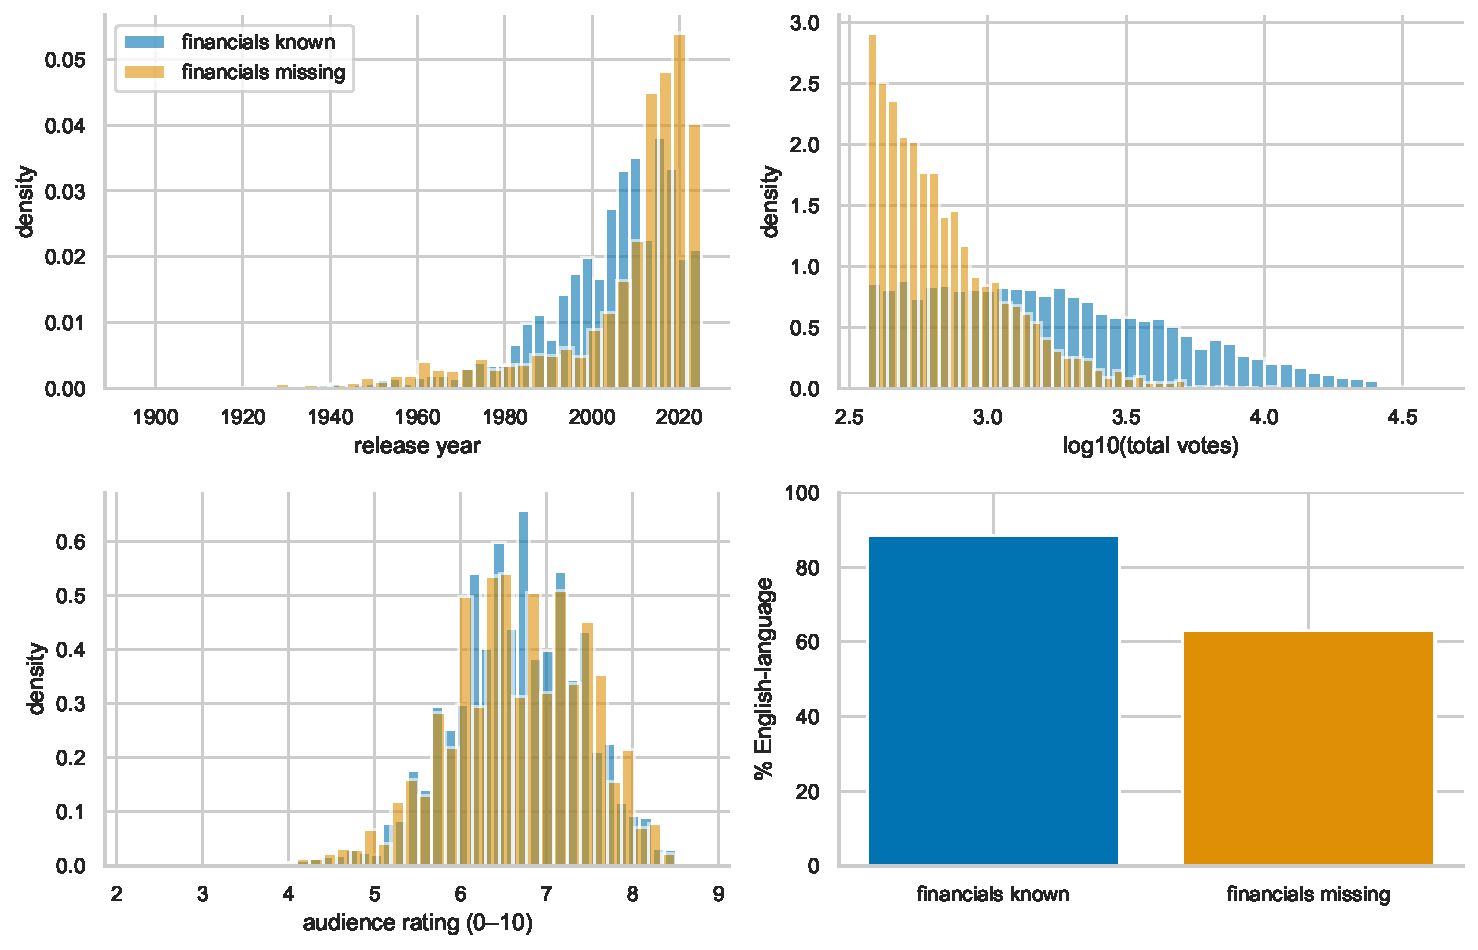
\includegraphics[width=\linewidth]{fig2_2_mar_comparison}
\caption{Documented (blue) against undocumented (orange) films. Undocumented films are concentrated in the most recent years, have far fewer votes and are less often in English. Their rating distribution is almost identical. What the undocumented films lack is commercial visibility, not quality.}
\label{fig:mar}
\end{figure}

The results are clear-cut, and one of them contradicts what we expected:

\begin{itemize}
  \item \textbf{Votes and popularity.} Undocumented films have a median of \CleanMarMedianVotesUndoc{} votes against \CleanMarMedianVotesDoc{} ($p\,\CleanMarPVotes$), and are less popular ($p\,\CleanMarPVotes$).
  \item \textbf{Language.} \CleanMarPctEnglishUndoc\% of undocumented films are in English, against \CleanMarPctEnglishDoc\% of documented ones ($p=\CleanMarPLanguage$).
  \item \textbf{Release year.} We expected undocumented films to be \emph{older}; they are \emph{newer}, with a median release year of \CleanMarMedianYearUndoc{} against \CleanMarMedianYearDoc{} ($p=\CleanMarPYear$). The gap comes from recent, small, often non-English or streaming-era releases whose box office is never published.
  \item \textbf{Audience rating.} This is the only variable on which the groups do not differ significantly ($p=\CleanMarPRating$).
\end{itemize}

The missingness is therefore not MCAR. At best it is \emph{missing at random} (MAR): explained by votes, popularity, language and year. Plausibly it is \emph{missing not at random} (MNAR): films that earned little may be exactly the ones whose figures go unreported.

\section{Imputation}

\paragraph{Decision: complete-case analysis for financial questions, no imputation of money.} A median budget filled into the undocumented films would invent plausible-looking numbers for precisely the films least like the ones the median was computed from. A group-wise or model-based imputation would need the missingness to be explained by observed variables (MAR), which we cannot verify and have reason to doubt. So we do not impute budget or revenue anywhere. Every financial statistic is computed on the films where both figures are known, and the sample size is stated beside it.

\paragraph{The cost of this choice, stated once and plainly.} Financial conclusions in this report apply to \emph{well-documented, mostly mainstream, mostly English-language} films, not to cinema in general. Conclusions about ratings use all \CleanRowsOut{} cleaned films and are not limited in this way.

\paragraph{Where imputation is used.} The modelling pipelines in Chapter~\ref{ch:models} fill the few missing non-financial inputs (runtime, director history) with medians or the most frequent category. These are fitted on the training years only, inside a \code{Pipeline}, so no information from the test years leaks in.

\section{Other defects and how each was handled}

\paragraph{Implausible values.} Budgets or revenues between \$1 and \$999 are data-entry errors or figures recorded in thousands. We set a floor of \$1{,}000 and converted the \CleanBudgetFloored{} budgets and \CleanRevenueFloored{} revenues below it to missing, rather than dropping the films. One runtime of zero minutes and one director recorded as the literal string ``Name'' (a scraping placeholder) were also converted to missing.

\paragraph{Duplicates.} \AuditExactDuplicateRows{} rows are exact copies of another row and were dropped. The audit found \AuditDuplicatedTitles{} repeated titles. Most are legitimate remakes released in different years, so title alone is not a duplicate key. Even title plus year is not safe: of the \AuditDuplicatedTitleYear{} repeated (title, year) pairs, only the exact copies are errors. The rest are genuinely different films, such as two different 2011 versions of \emph{War of the Buttons} with different directors and runtimes, or two unrelated 2026 films called \emph{The Odyssey}. Deduplicating on title plus year would have deleted real films.

\paragraph{Categories.} \code{Unrated} and \code{NR} mean the same thing, so the \CleanContentRatingNrMerged{} \code{NR} films were merged into \code{Unrated}. A stray rating stored as \code{"PG-13~"} (with a trailing space) was stripped. ``United States of America'' was shortened to ``United States'' inside \CleanCountryRowsRenamed{} country strings, so that country counts are not split by spelling.

\paragraph{Dates.} Release dates are stored as month/day/year, except for two Lumi\`ere films from the 1890s stored as year-month-day. The loader parses both formats, leaving the \AuditPrimaryNullReleaseDate{} genuinely missing dates.

\paragraph{Unreleased films.} \CleanFutureFlagged{} films are dated after 2025. Their revenue is necessarily incomplete, so they are flagged and excluded from every revenue and ROI analysis. They stay in the file for descriptive counts.

\section{Joining the secondary dataset}\label{sec:secondary}

The Kaggle file was joined on normalised title (trimmed, case-folded) plus release year. \CleanSecondaryMatched{} primary rows found a match. The join served its three permitted purposes:

\begin{itemize}
  \item \textbf{Join key.} The TMDB \code{id} is now attached to every matched film.
  \item \textbf{Cross-validation.} On the \CleanCrossvalN{} matched films, the scraped audience rating and Kaggle's vote average agree almost perfectly: Pearson $r=\CleanCrossvalRatingPearson$, Spearman $r=\CleanCrossvalRatingSpearman$ (Figure~\ref{fig:crossval}). This is strong evidence that the scrape itself is sound. Popularity agrees less closely (Spearman $r=\CleanCrossvalPopularitySpearman$), as expected: TMDB popularity is a time-varying engagement score, and the two files were collected at different dates.
  \item \textbf{Filling gaps.} The genre and overview fill filled nothing (\CleanGenresFilled{} values). The only primary rows missing a genre or overview are obscure films all titled \emph{Return}, none of which appears in Kaggle's top-10{,}000 list. We report this rather than imply the secondary file helped.
\end{itemize}

\begin{figure}[htbp]
\centering
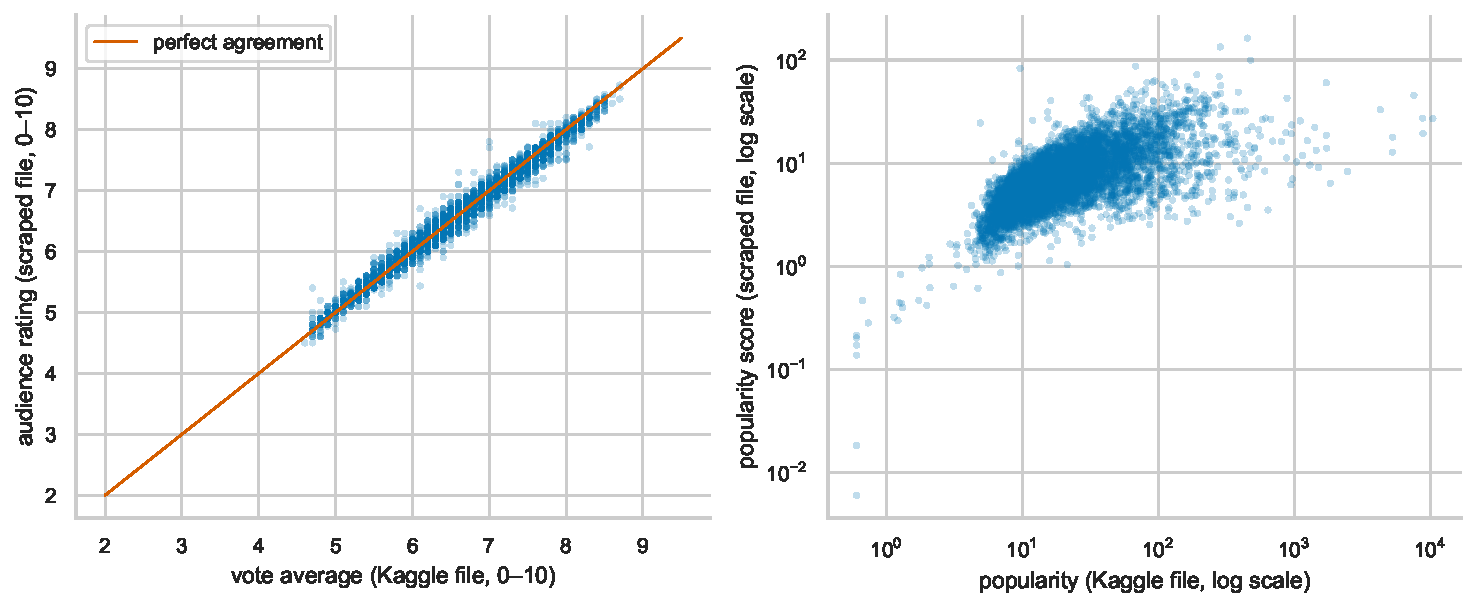
\includegraphics[width=\linewidth]{fig2_3_crossval}
\caption{Cross-source validation on \CleanCrossvalN{} matched films. Left: ratings from the two collections lie almost exactly on the line of perfect agreement, so the scraped ratings can be trusted. Right: popularity agrees only loosely, consistent with a time-sensitive score sampled at two different dates.}
\label{fig:crossval}
\end{figure}

\section{Inflation adjustment}

Budgets and revenues are in nominal dollars across 1895--2026, and a 1975 dollar and a 2023 dollar are not the same amount of money. Both columns were deflated to constant \CleanCpiBaseYear{} dollars using the annual average of the CPI:
\begin{equation}
  X^{(2025)}_i \;=\; X^{\text{nominal}}_i \times \frac{\text{CPI}_{2025}}{\text{CPI}_{\text{year}(i)}} .
\end{equation}
As a check: \emph{Jaws} (1975) cost \$\CleanDeflateJawsNominalM{}M nominal, or \$\CleanDeflateJawsTwoZeroTwoFiveM{}M in 2025 dollars. \emph{Titanic} (1997) cost \$\CleanDeflateTitanicNominalM{}M, or \$\CleanDeflateTitanicTwoZeroTwoFiveM{}M. \emph{Oppenheimer} (2023) cost \$\CleanDeflateOppenheimerNominalM{}M, or \$\CleanDeflateOppenheimerTwoZeroTwoFiveM{}M.

The CPI series starts in 1913, so films released earlier get no deflated value rather than an invented one. None of them has usable financials (\CleanDeflationLostUsable{} films in the financial sample are affected). Return on investment is a ratio of two same-year amounts, so the inflation factor cancels and ROI is identical whether nominal or deflated dollars are used.

\section{Reconciliation}

Table~\ref{tab:recon} accounts for every row. \CleanRowsIn{} rows come in, and \CleanRowsOut{} leave the cleaning stage after the exact duplicates are dropped. Of those, \CleanUsableFinancialSample{} films have both financials known and plausible and are released by 2025. That is the sample for every financial analysis that follows.

\begin{table}[htbp]
\centering\small
\tablein{tab2_4_reconciliation}
\caption{Row reconciliation. Only exact duplicates are removed; the financial sample is a flagged subset, not a separate file.}
\label{tab:recon}
\end{table}

%%%%%%%%%%%%%%%%%%%%%%%%%%%%%%%%%%%%%%%%%%%%%%%%%%%%%%%%%%%%%%%%%%%%%%%%%%%
\chapter{Visualization}\label{ch:viz}
%%%%%%%%%%%%%%%%%%%%%%%%%%%%%%%%%%%%%%%%%%%%%%%%%%%%%%%%%%%%%%%%%%%%%%%%%%%

All figures share one plotting style, chosen to be readable by colour-blind readers. Every axis carries units, and variables that span several orders of magnitude are drawn on log scales labelled as such. Financial figures use the \UniNFinancial{}-film financial sample; all others use the \UniNAll{} cleaned films. Each caption states the sample size and what the reader should notice.

\section{Univariate analysis}

\subsection{Budget and revenue}

Figure~\ref{fig:moneydist} shows budget and revenue on both linear and log scales. The linear panels are kept on purpose: they show why the log scale is needed. Both variables are extremely right-skewed (skewness \UniBudgetSkew{} for budget and \UniRevenueSkew{} for revenue). The median budget is \$\UniBudgetMedianM{}M and the median revenue \$\UniRevenueMedianM{}M, both nominal.

\begin{figure}[htbp]
\centering
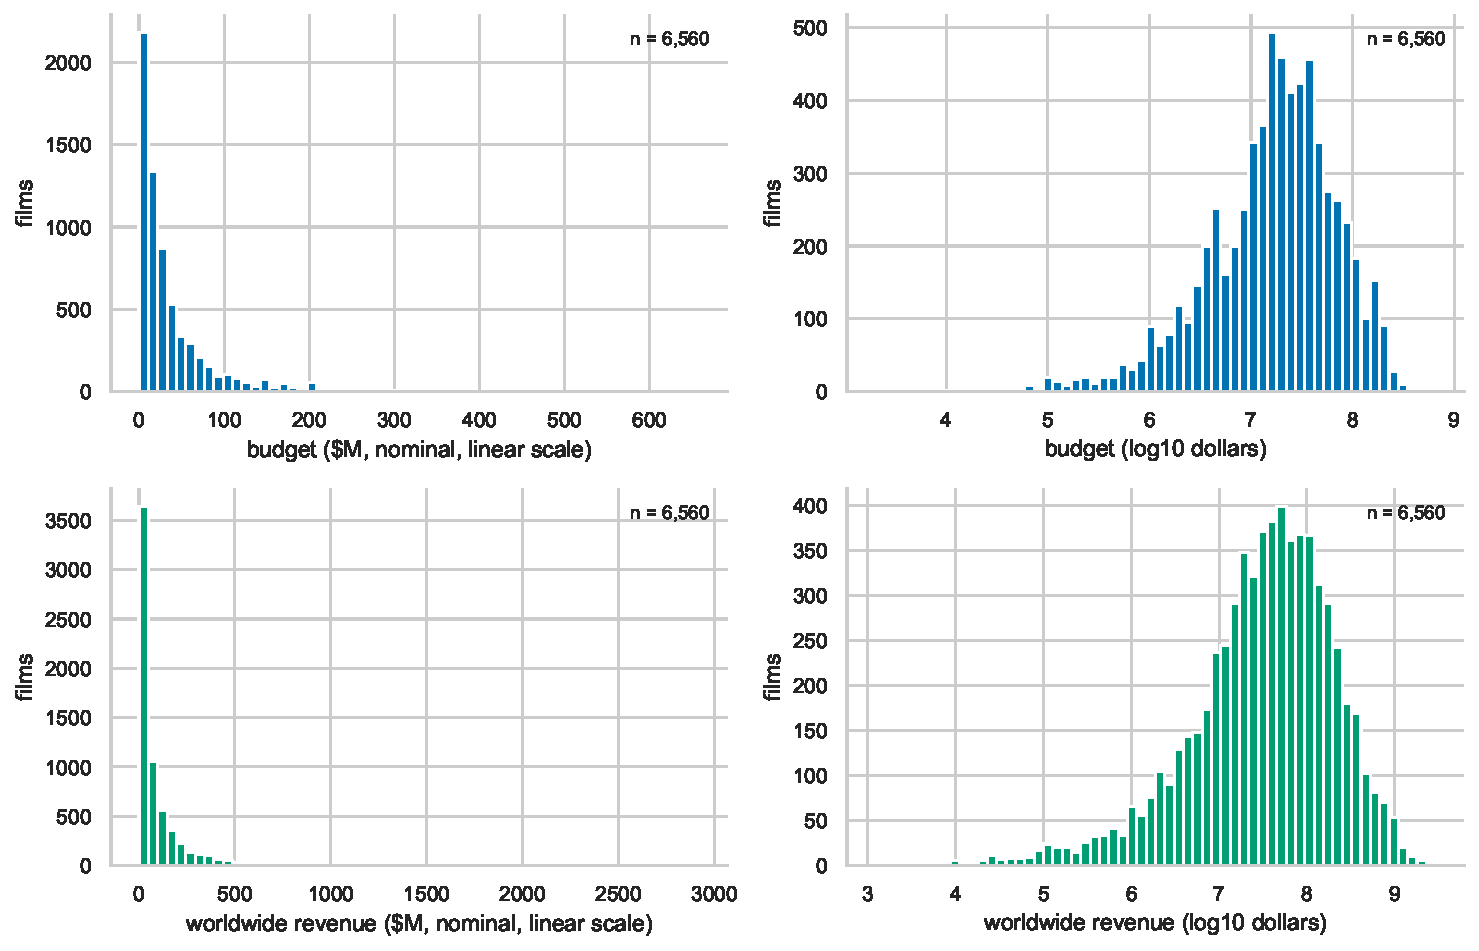
\includegraphics[width=\linewidth]{fig3_1_budget_revenue_dist}
\caption{Budget (top) and worldwide revenue (bottom), on linear (left) and log (right) scales, $n=\UniNFinancial$. On the linear scale almost every film is squashed against zero by a handful of blockbusters. On the log scale both are far closer to symmetric, which is why every later financial plot uses log axes and every model uses log-transformed money.}
\label{fig:moneydist}
\end{figure}

\subsection{Runtime, rating and release year}

\begin{figure}[htbp]
\centering
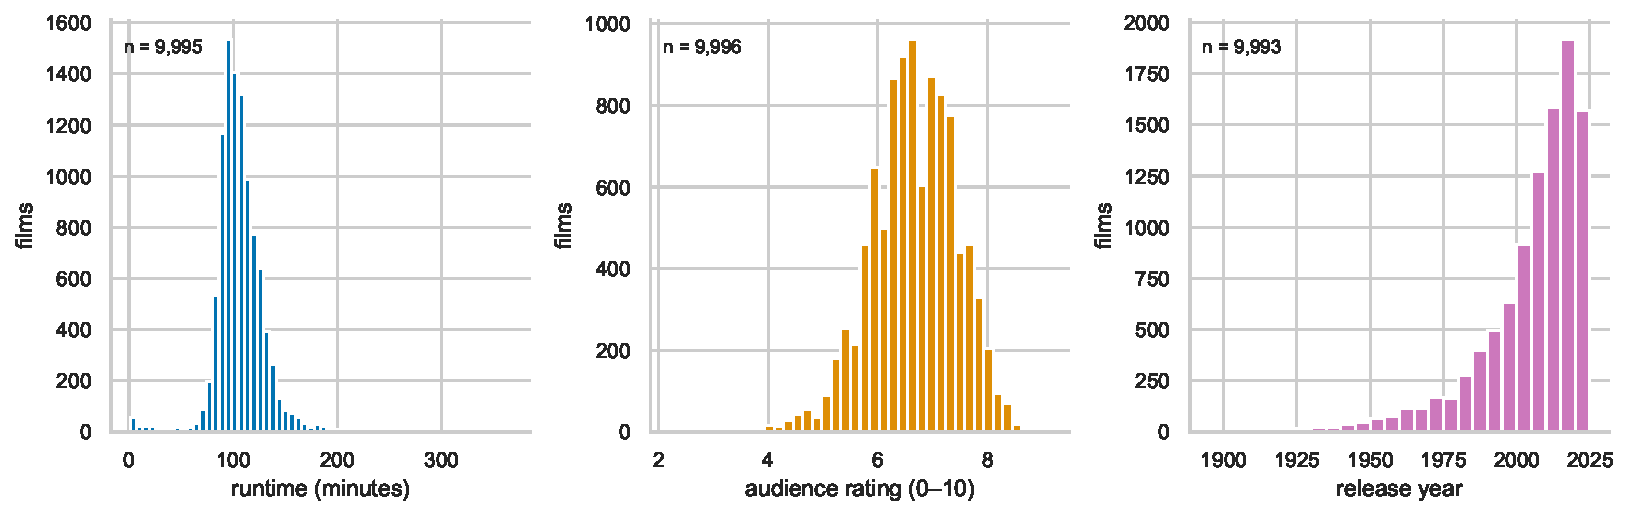
\includegraphics[width=\linewidth]{fig3_2_runtime_rating_year_dist}
\caption{Runtime, audience rating and release year, all cleaned films. Runtime clusters around a median of \UniRuntimeMedian{} minutes, with a long tail of epics. Ratings are close to symmetric around a mean of \UniRatingMean{}, because the vote filter has already removed the obscure films that attract the lowest ratings. Release years pile up after 1990, so this is overwhelmingly a collection of modern films.}
\label{fig:otherdist}
\end{figure}

Figure~\ref{fig:otherdist} shows that runtime is only mildly skewed (skewness \UniRuntimeSkew), so it needs no transformation. Ratings are slightly left-skewed (skewness \UniRatingSkew). \UniPctFilmsSinceOneNineNineZero\% of all films, and \UniPctFinSinceOneNineNineZero\% of the financial sample, were released in 1990 or later (Figure~\ref{fig:peryear}).

\begin{figure}[htbp]
\centering
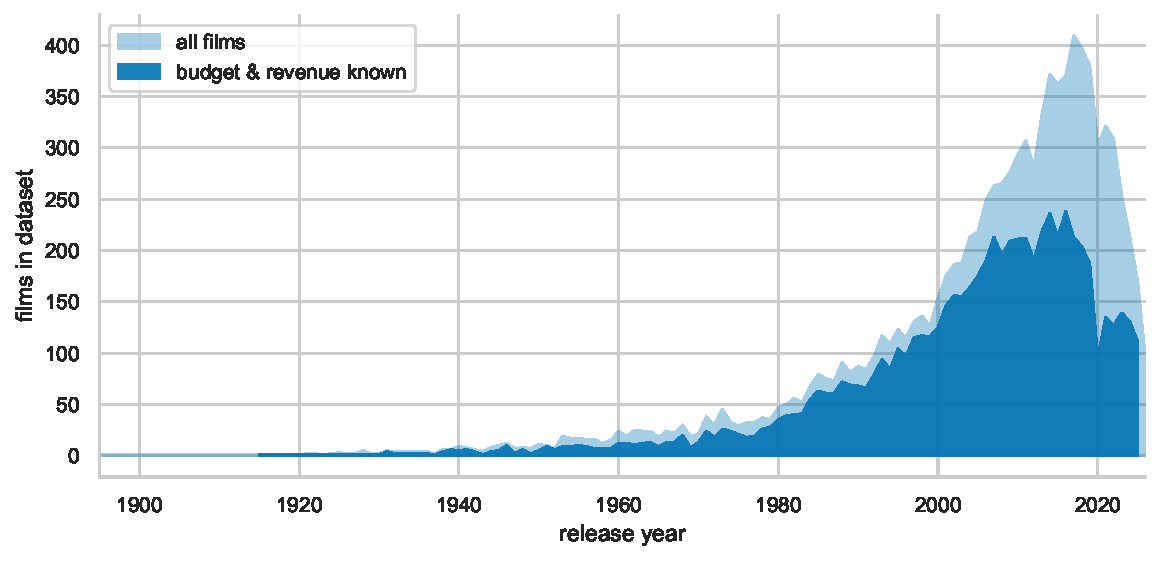
\includegraphics[width=0.9\linewidth]{fig3_3_films_per_year}
\caption{Films per release year: all films (light) and films with both financials known (dark). The financial sample follows the shape of the whole collection until the most recent years, when the gap between the two widens. That widening is the recent-film missingness found in Chapter~\ref{ch:cleaning}.}
\label{fig:peryear}
\end{figure}

\subsection{Genre, language and content rating}

Genres are multi-label: a film tagged ``Action, Adventure'' carries both labels, and the order inside the string is meaningless. Read as raw strings, the column has \UniNGenreCombinationsRaw{} distinct ``categories''. Split into individual labels, it has \UniNGenres{} genres. We always split, so a film counts once under each of its genres and the genre bars in Figure~\ref{fig:genrelang} add up to more than the number of films. \UniTopGenre{} is the most common genre, carried by \UniTopGenreCount{} films.

\begin{figure}[htbp]
\centering
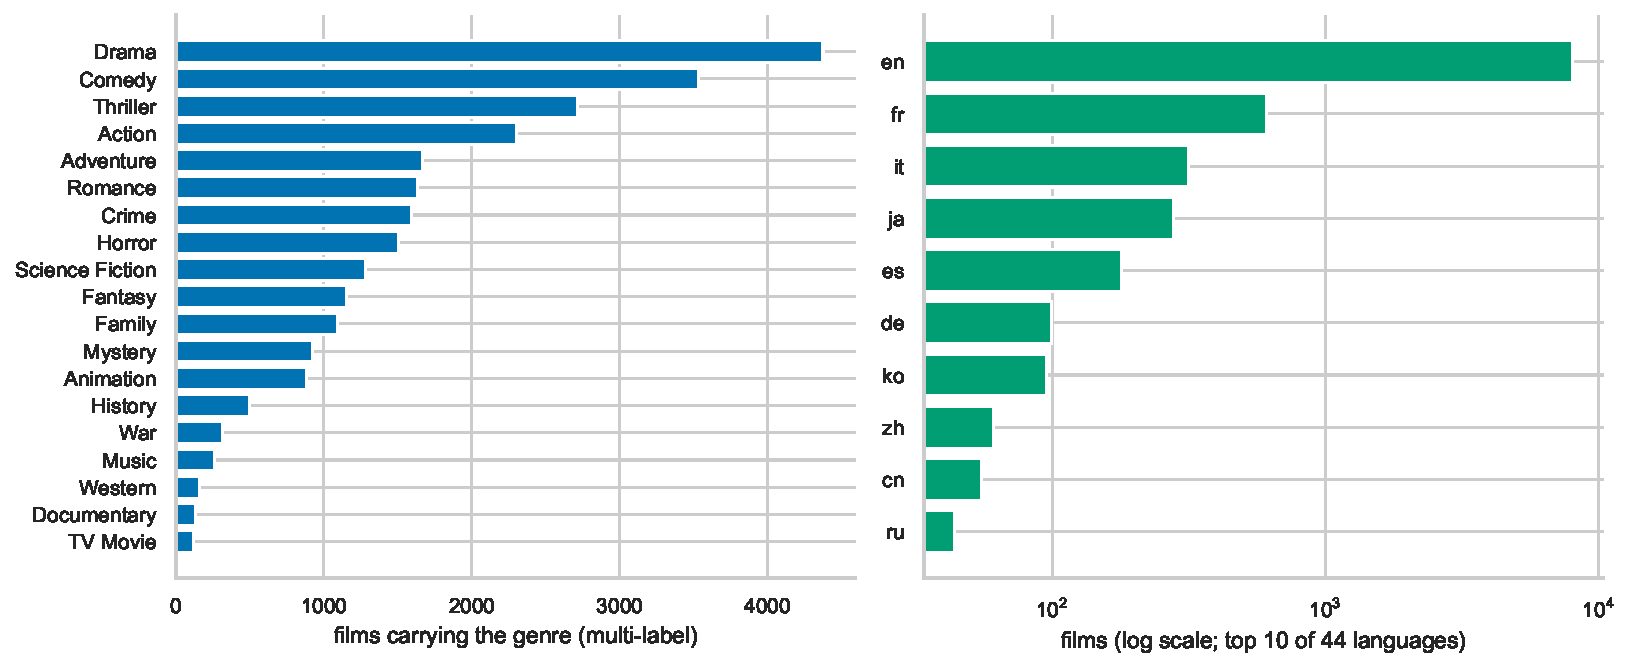
\includegraphics[width=\linewidth]{fig3_4_genre_language_freq}
\caption{Left: films carrying each genre (multi-label, split into individual genres). Right: the ten most common original languages, on a log scale because English dominates. English outnumbers the second language (\UniSecondLanguage, French) by \UniEnglishToSecondRatio{} to one, a reminder of how Anglophone this sample is.}
\label{fig:genrelang}
\end{figure}

\begin{figure}[htbp]
\centering
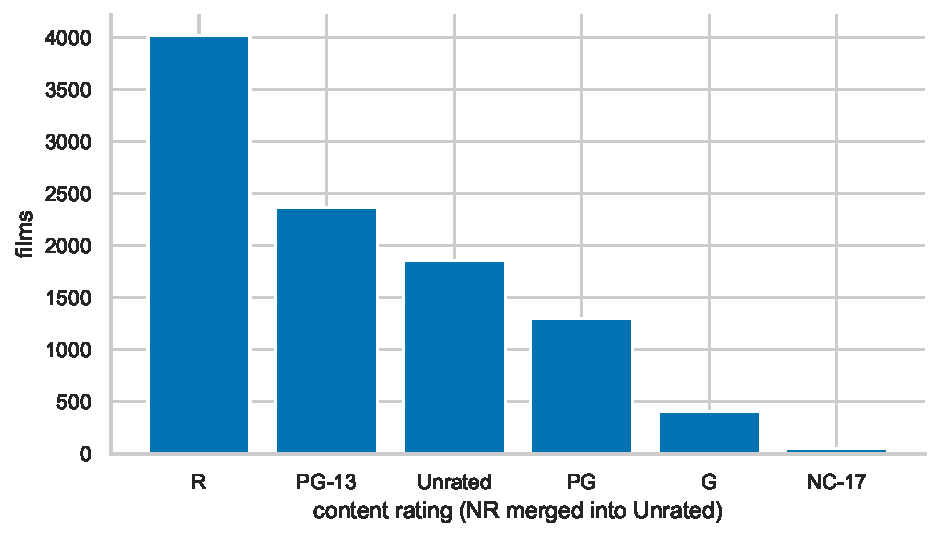
\includegraphics[width=0.75\linewidth]{fig3_5_content_rating}
\caption{Content ratings after \code{NR} was merged into \code{Unrated}. \UniTopContentRating{}-rated films are the largest group (\UniTopContentRatingCount{} films). \code{Unrated} means only that a film never received a US rating; it says nothing about the film's content.}
\label{fig:cr}
\end{figure}

\section{Multivariate analysis}

\subsection{Budget against revenue}

\begin{figure}[htbp]
\centering
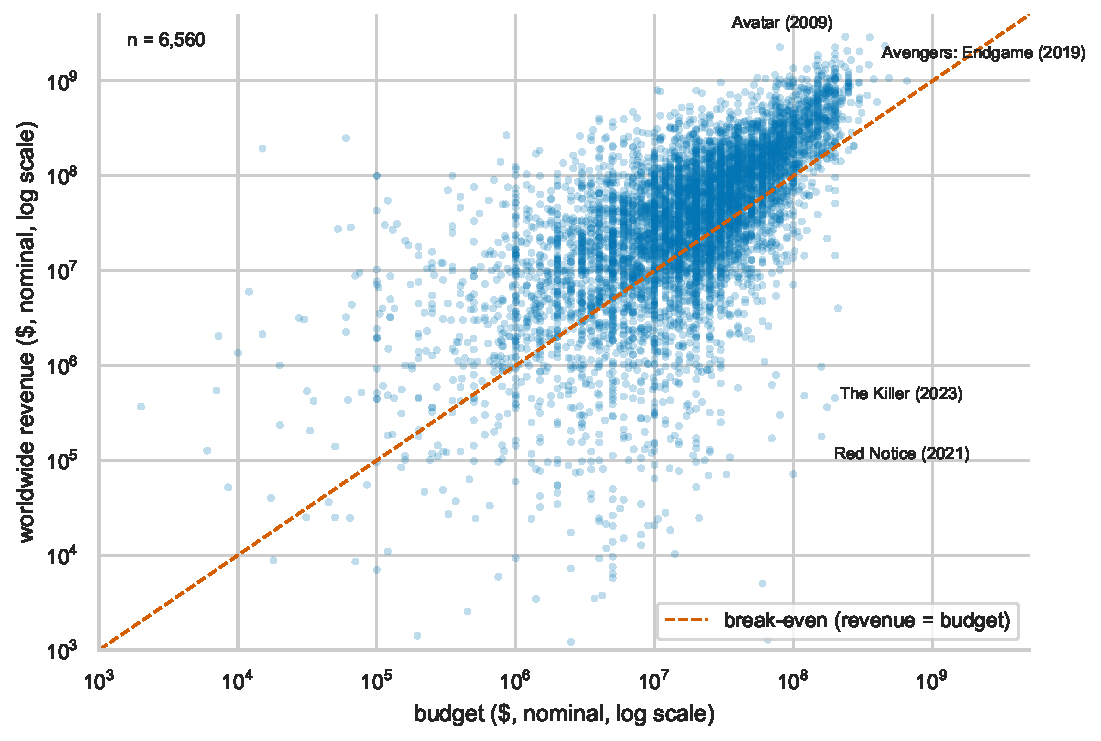
\includegraphics[width=0.92\linewidth]{fig3_6_budget_vs_revenue}
\caption{Budget against worldwide revenue on log--log axes, $n=\MultiNFinancial$. Films below the dashed line did not recoup even their production budget from worldwide gross; that is \MultiPctBelowBreakeven\% of documented films, before marketing costs are counted. The two highest grosses and the two big-budget films furthest below the line are labelled. The latter, \MultiFlopTitleA{} and \MultiFlopTitleB{}, are streaming originals: their recorded ``revenue'' is not box office. The vertical stripes are budgets reported as round numbers.}
\label{fig:budrev}
\end{figure}

Budget and revenue are strongly associated: Pearson $r=\MultiBudgetRevenuePearsonLoglog$ on the log scale and Spearman $r=\MultiBudgetRevenueSpearman$ ($p\,\MultiBudgetRevenuePearsonP$, $n=\MultiNFinancial$). Figure~\ref{fig:budrev} also shows how wide the scatter is. At any given budget, revenue spans two to three orders of magnitude.

The plot exposes two data-quality issues worth naming. First, \MultiPctBudgetsRoundMillion\% of budgets are exact multiples of \$1M, so many budgets are rounded estimates rather than accounts. Second, streaming originals appear with token revenue figures. They look like catastrophic flops, but their ``revenue'' measures something different from box office. Both issues add noise to every financial result.

\subsection{Return on investment by genre}

We define return on investment as
\begin{equation}
  \text{ROI}_i = \frac{\text{revenue}_i}{\text{budget}_i},
\end{equation}
so a film breaks even on its production budget at $\text{ROI}=1$. Figure~\ref{fig:roigenre} and Table~\ref{tab:roigenre} compare genres. Each genre's ROI is shown beside its budget distribution, because averaging ROI across genres invites Simpson's paradox: a genre made cheaply can post huge ratios on tiny denominators.

\begin{figure}[htbp]
\centering
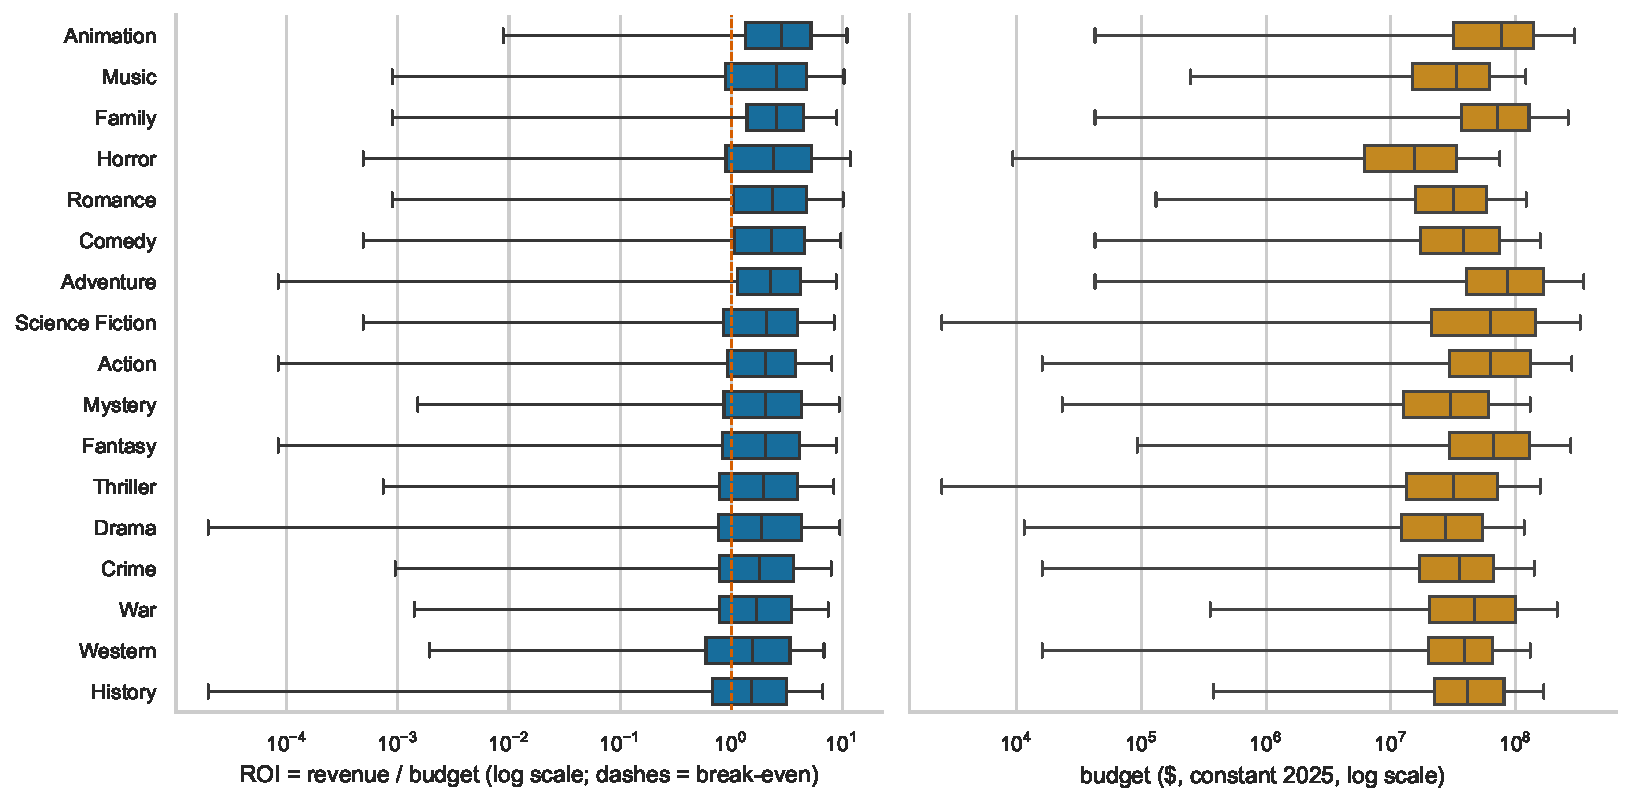
\includegraphics[width=\linewidth]{fig3_7_roi_by_genre}
\caption{ROI by genre, ordered by median (left), next to each genre's budget distribution in constant 2025 dollars (right). Genres with at least \MultiGenreMinN{} documented films; films count in each of their genres. \MultiGenreTopMedianRoi{} has the highest median ROI despite one of the largest budgets. Horror, the folk favourite, sits mid-table on the smallest budgets.}
\label{fig:roigenre}
\end{figure}

\begin{table}[htbp]
\centering\small
\tablein{tab3_1_roi_by_genre}
\caption{ROI by genre: median beside mean. The mean exceeds the median in every genre, and wildly so for Horror and Mystery.}
\label{tab:roigenre}
\end{table}

This result contradicts the common belief that horror is the most profitable genre. By median ROI, \MultiGenreTopMedianRoi{} leads (\MultiGenreTopMedianRoiValue), followed by Music and Family. Horror is mid-table at \MultiHorrorMedianRoi, on a median budget of only \$\MultiHorrorMedianBudgetM{}M against Animation's \$\MultiAnimationMedianBudgetM{}M.

Horror's reputation rests on its \emph{mean} ROI of \MultiHorrorMeanRoi. That mean is inflated by two micro-budget phenomena, \emph{Paranormal Activity} and \emph{The Blair Witch Project}, each with an ROI in the thousands. Both are also tagged Mystery, which is why Mystery's mean (\MultiMysteryMeanRoi) is even further from its median (\MultiMysteryMedianRoi). Reported alone, mean ROI by genre would be badly misleading.

\subsection{Rating against revenue}

\begin{figure}[htbp]
\centering
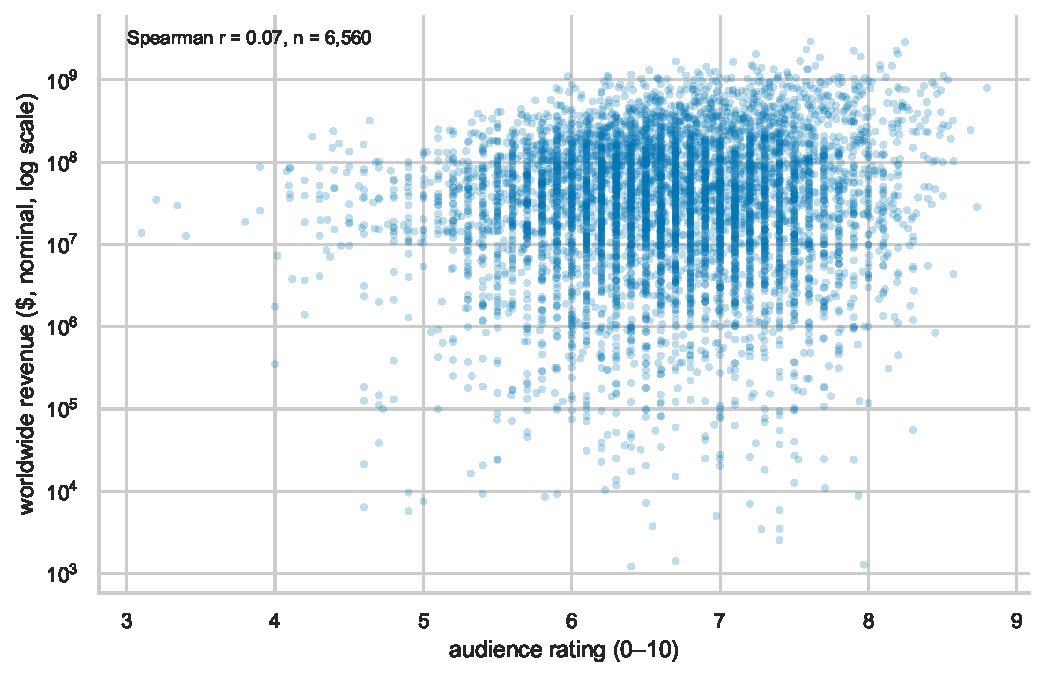
\includegraphics[width=0.85\linewidth]{fig3_8_rating_vs_revenue}
\caption{Audience rating against worldwide revenue, $n=\MultiNFinancial$. The cloud has almost no slope (Spearman $r=\MultiRatingRevenueSpearman$): highly rated films are not systematically higher-grossing, and low-rated films are not systematically lower-grossing.}
\label{fig:ratrev}
\end{figure}

Audience rating and revenue are almost unrelated (Figure~\ref{fig:ratrev}): Spearman $r=\MultiRatingRevenueSpearman$, $p=\MultiRatingRevenueP$, $n=\MultiNFinancial$. The association is statistically detectable only because the sample is large; in practical terms it is negligible. This is a substantive finding: critical and commercial success are largely different outcomes.

\subsection{Release month}

\begin{figure}[htbp]
\centering
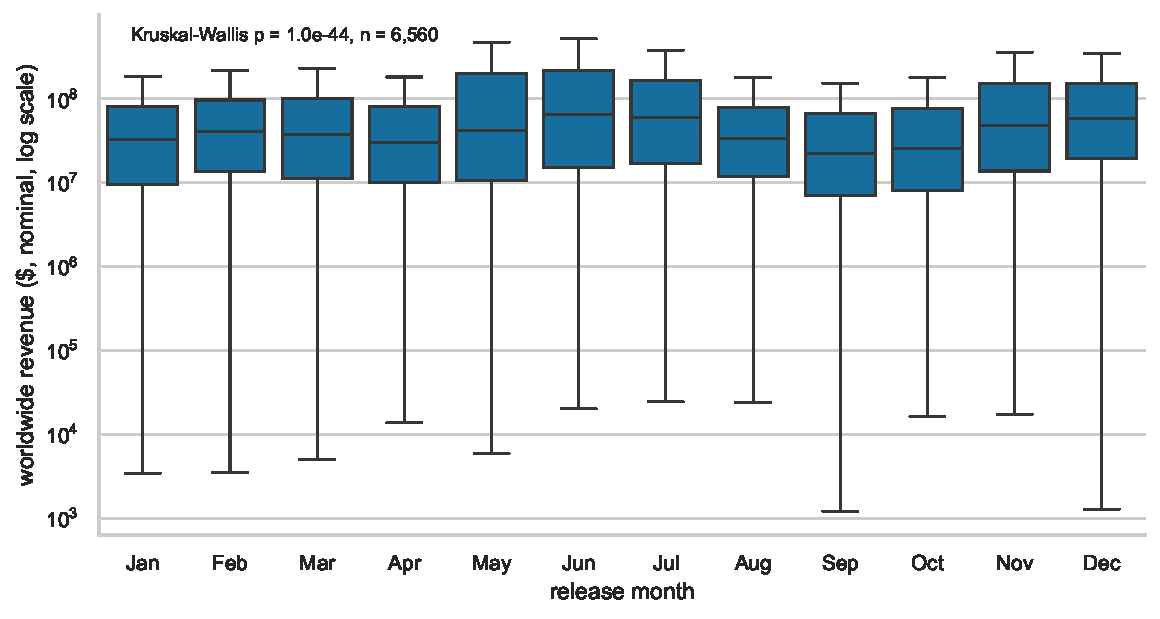
\includegraphics[width=0.92\linewidth]{fig3_9_month_vs_revenue}
\caption{Worldwide revenue by release month (box plots, log scale), $n=\MultiNMonth$. June, July and December lead; September and October trail. The summer and winter-holiday windows show up clearly in the data.}
\label{fig:month}
\end{figure}

Revenue differs by release month (Kruskal--Wallis $p=\MultiMonthKruskalP$, $n=\MultiNMonth$; Figure~\ref{fig:month}). The median \MultiBestMonthName{} release earned \$\MultiBestMonthMedianM{}M and the median \MultiWorstMonthName{} release \$\MultiWorstMonthMedianM{}M, a ratio of \MultiJuneToSeptemberRatio. July (\$\MultiJulyMedianM{}M) and December (\$\MultiDecemberMedianM{}M) follow June. Studios choose release dates, and they hold their biggest films for these windows, so this association mixes any genuine seasonal effect with the selection of which films are released when.

\subsection{Correlations among numeric variables}

\begin{figure}[htbp]
\centering
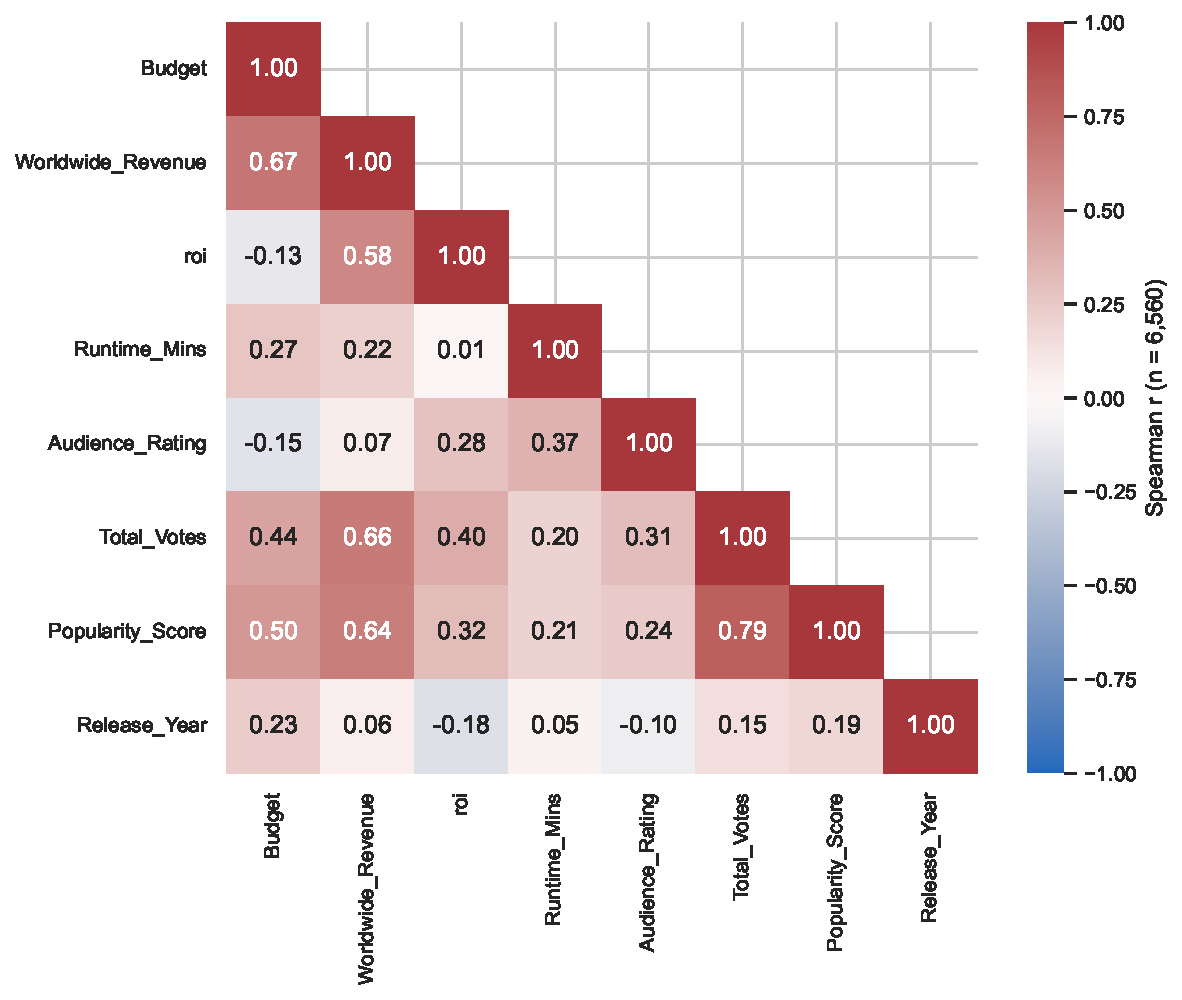
\includegraphics[width=0.82\linewidth]{fig3_10_corr_heatmap}
\caption{Spearman correlations among numeric variables, $n=\MultiNFinancial$ for every cell. Votes and popularity track revenue closely, but both are recorded \emph{after} release, so they cannot explain success, only reflect it. ROI is weakly \emph{negative} against budget.}
\label{fig:corr}
\end{figure}

We use Spearman correlations because the financial variables are too skewed for Pearson correlation to be meaningful (Figure~\ref{fig:corr}). Two cells matter most for what follows:
\begin{itemize}
  \item \textbf{Votes and revenue} correlate at $r=\MultiVotesRevenueSpearman$. Votes accumulate after release, so this is a symptom of success rather than an attribute a studio could choose. Chapter~\ref{ch:features} excludes votes from all models for this reason.
  \item \textbf{ROI and budget} correlate at $r=\MultiRoiBudgetSpearman$ ($p=\MultiRoiBudgetSpearmanP$): bigger budgets go with \emph{lower} returns per dollar.
\end{itemize}

\subsection{Runtime against rating}

\begin{figure}[htbp]
\centering
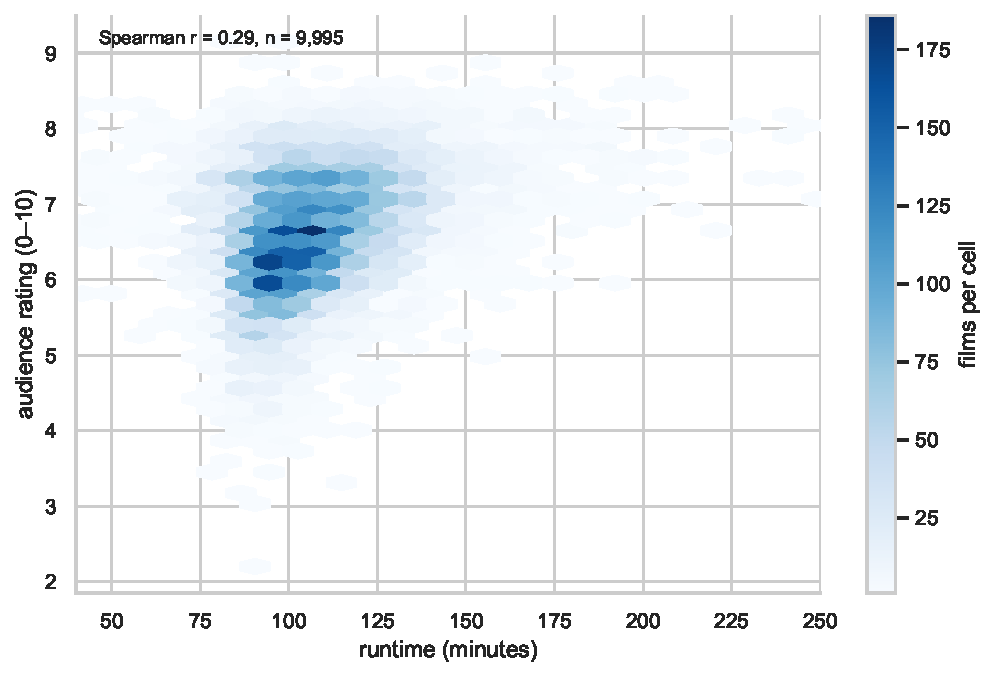
\includegraphics[width=0.82\linewidth]{fig3_11_runtime_vs_rating}
\caption{Runtime against audience rating (hexagonal bins), $n=\MultiRuntimeRatingN$. Longer films are rated modestly higher (Spearman $r=\MultiRuntimeRatingSpearman$), but at every runtime ratings spread over several points.}
\label{fig:runrat}
\end{figure}

Longer films receive modestly higher ratings: Spearman $r=\MultiRuntimeRatingSpearman$, $p=\MultiRuntimeRatingP$, $n=\MultiRuntimeRatingN$ (Figure~\ref{fig:runrat}). A plausible reading is selection rather than length itself: long runtimes are granted to prestige dramas and epics, which are rated well, while short runtimes are typical of genre fare.

\subsection{Budget and ROI over the decades}

\begin{figure}[htbp]
\centering
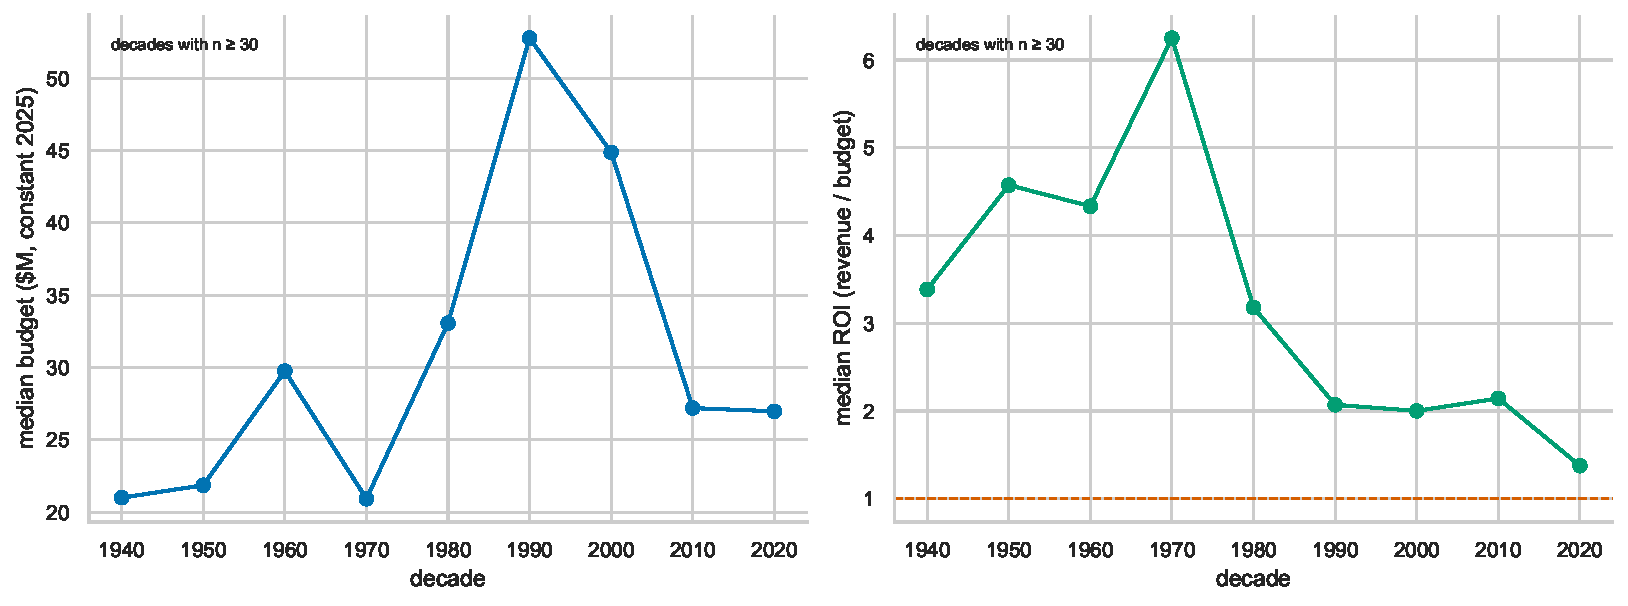
\includegraphics[width=\linewidth]{fig3_12_decade_trends}
\caption{Median budget in constant 2025 dollars (left) and median ROI (right) by decade, for decades with at least 30 documented films. Real budgets peaked in the 1990s and have fallen since, while median ROI has fallen from its 1970s peak. The very high ROI of the 1950s--1970s is partly survivorship: an old film is in this dataset only if it is still rated today, which favours the hits of its era.}
\label{fig:decades}
\end{figure}

\begin{table}[htbp]
\centering\small
\tablein{tab3_2_decades}
\caption{Median budget (constant 2025 dollars) and median ROI by decade. The decades before 1940 hold too few documented films to interpret.}
\label{tab:decades}
\end{table}

Median real budgets rose from \$\MultiDecadeOneNineSevenZeroMedianBudgetM{}M in the 1970s to a peak of \$\MultiDecadeOneNineNineZeroMedianBudgetM{}M in the 1990s, then fell back to \$\MultiDecadeTwoZeroOneZeroMedianBudgetM{}M in the 2010s (Figure~\ref{fig:decades}, Table~\ref{tab:decades}). Median ROI fell from \MultiDecadeOneNineSevenZeroMedianRoi{} in the 1970s to \MultiDecadeOneNineNineZeroMedianRoi{} in the 1990s, held roughly level through the 2010s (\MultiDecadeTwoZeroOneZeroMedianRoi), then dropped to \MultiDecadeTwoZeroTwoZeroMedianRoi{} in the 2020s ($n=\MultiDecadeTwoZeroTwoZeroN$). Two cautions apply. The early decades are flattered by survivorship. The 2020s include both the pandemic collapse of cinema-going and recent releases whose revenue may not yet be complete on TMDB.

\subsection{Two questions from Chapter~\ref{ch:intro}}

\paragraph{Rating per dollar, by genre.} For each genre with at least 100 documented films, Figure~\ref{fig:value} plots median rating against median budget, and Table~\ref{tab:value} gives the ratio of the two. Two results stand out:
\begin{itemize}
  \item \textbf{Rating per dollar.} \MultiValueTopGenre{} gives the most rating per \$10M of median budget (\MultiValueTopRatio), followed by \MultiValueSecondGenre. \MultiValueBottomGenre{} gives the least (\MultiValueBottomRatio).
  \item \textbf{No evidence that cost and rating are related across genres.} Spending more is not what makes a genre well rated: Spearman $r=\MultiGenreBudgetRatingSpearman$, $p=\MultiGenreBudgetRatingP$, $n=\MultiGenreBudgetRatingN$ genres. \MultiValueTopRatingGenre{} films have the highest median rating (\MultiValueTopRating) on a middling budget.
\end{itemize}
A ratio like this is dominated by its denominator, so the scatter is the more honest picture: horror tops the ratio because it is cheap, not because it is well rated. It has the \emph{lowest} median rating of any genre.

\begin{figure}[htbp]
\centering
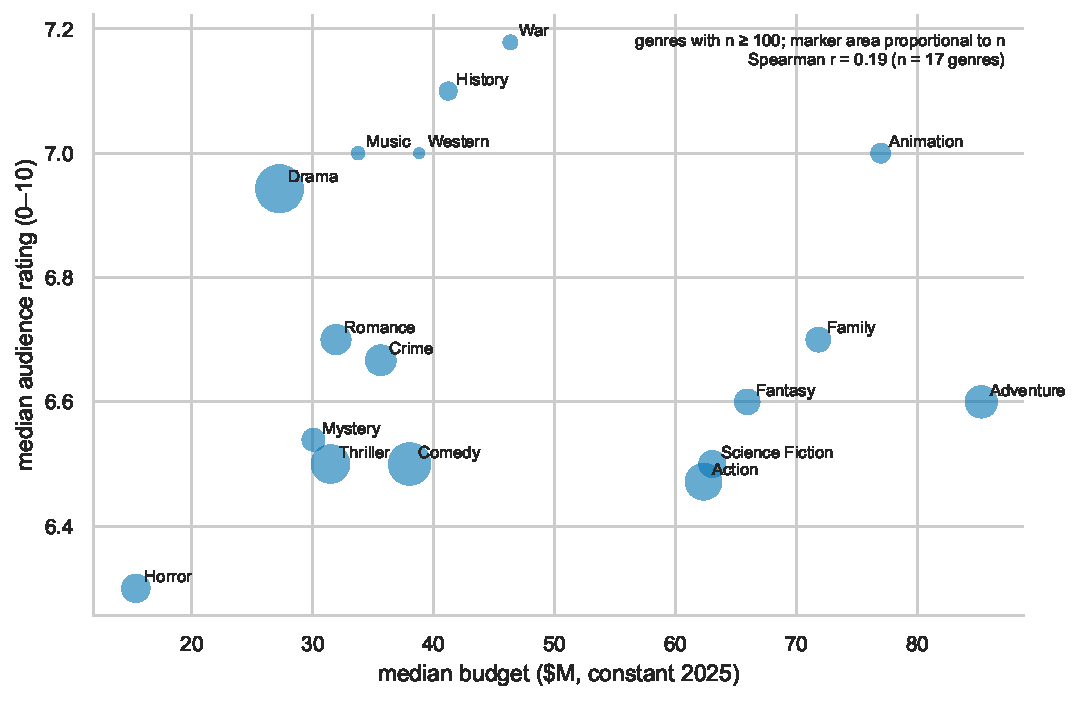
\includegraphics[width=0.88\linewidth]{fig3_13_genre_value}
\caption{Median audience rating against median budget (constant 2025 dollars) per genre; marker area is proportional to the number of films. Genres towards the top left give the most rating for the least money. There is no overall slope: across genres, higher budgets are not associated with higher ratings.}
\label{fig:value}
\end{figure}

\begin{table}[htbp]
\centering\small
\tablein{tab3_3_genre_value}
\caption{Median rating, median budget and rating per \$10M of budget, by genre, ordered by the ratio.}
\label{tab:value}
\end{table}

\paragraph{Mid-budget films since 2000.} We fixed the definition of ``mid-budget'' before looking at outcomes: a budget between \$20M and \$80M in 2025 dollars. That gives \MultiMidN{} films released from 2000 onwards (Table~\ref{tab:mid}).
\begin{itemize}
  \item \textbf{2000s to 2010s: no change.} Median ROI went from \MultiMidRoiTwoZeroZeroZeros{} to \MultiMidRoiTwoZeroOneZeros{}, and the profitable share from \MultiMidPctProfTwoZeroZeroZeros\% to \MultiMidPctProfTwoZeroOneZeros\%. The difference is not significant (Mann--Whitney $p=\MultiMidTwoZeroZeroZerosVsTwoZeroOneZerosP$).
  \item \textbf{2020--25: a sharp fall.} Median ROI is \MultiMidRoiTwoZeroTwoZeros{} and only \MultiMidPctProfTwoZeroTwoZeros\% are profitable. Across all three periods the differences are significant (Kruskal--Wallis $p=\MultiMidKruskalP$; chi-square on the profitable share, $p=\MultiMidChiTwoP$).
\end{itemize}

\begin{table}[htbp]
\centering\small
\tablein{tab3_4_mid_budget}
\caption{Mid-budget films (\$20M--\$80M in 2025 dollars) by period. Flat from the 2000s to the 2010s; a sharp fall in 2020--25.}
\label{tab:mid}
\end{table}

%%%%%%%%%%%%%%%%%%%%%%%%%%%%%%%%%%%%%%%%%%%%%%%%%%%%%%%%%%%%%%%%%%%%%%%%%%%
\chapter{Feature Engineering}\label{ch:features}
%%%%%%%%%%%%%%%%%%%%%%%%%%%%%%%%%%%%%%%%%%%%%%%%%%%%%%%%%%%%%%%%%%%%%%%%%%%

This chapter builds the variables the models in Chapter~\ref{ch:models} use, \FeatNEngineered{} engineered columns in all, and then tests which of them are worth keeping. One rule overrides convenience throughout: \textbf{a feature may only use information that would have been available before the film was released.}

\section{Feature extraction}

\begin{table}[htbp]
\centering\small
\begin{tabular}{>{\raggedright\arraybackslash}p{5.9cm}p{9.3cm}}
\toprule
feature & definition and reason \\
\midrule
\code{roi}, \code{profit}, \code{is\_profitable} & revenue/budget, revenue$-$budget, and ROI $>1$. These are \emph{targets}, never predictors. Missing wherever either financial value is missing. \\
\code{release\_month}, \code{\_quarter}, \code{\_decade} & Calendar position, from the parsed release date. \\
\code{is\_summer\_release}, \code{is\_holiday\_release} & May--July and November--December: the conventional industry windows, fixed in advance rather than tuned on outcomes. \\
\code{genre\_count}, \code{genre\_*} & Number of genres, and one 0/1 flag per genre (\UniNGenres{} flags). Order inside the genre string is ignored. \\
\code{is\_english} & Original language is English. \\
\code{director\_prior\_film\_count},\newline \code{director\_mean\_prior\_rating} & The director's earlier films in this dataset and their mean rating, using \emph{strictly earlier} releases only. \\
\code{studio\_tier} & major / mid / indie, from how often the film's best-connected production company appears in the data. \\
\code{overview\_length} & Characters in the synopsis, a rough proxy for how much was written about the film. \\
\bottomrule
\end{tabular}
\caption{Engineered features. Votes and popularity are kept for description but barred from every model, because both are recorded after release.}
\label{tab:features}
\end{table}

\paragraph{Director history without leakage.} A director's mean rating computed over their whole career would leak the future: it would use \emph{Oppenheimer}'s rating to describe \emph{Memento}. Each film's features are therefore computed only from the same director's films released strictly earlier. A director's first film in the data gets a count of zero and no prior rating. To verify the construction, we recomputed the feature from scratch for \FeatDirectorCheckN{} randomly chosen films and compared: \FeatDirectorCheckMatched{} of \FeatDirectorCheckN{} matched exactly. An assertion in the notebook makes any future regression fail loudly.

\paragraph{Studio tier.} Production companies were ranked by how many films in the cleaned data list them. Each film takes the tier of its most frequent company: \emph{major} if that company has at least 100 films, \emph{mid} if at least 20, and \emph{indie} otherwise. That gives \FeatStudioTierMajor{} major, \FeatStudioTierMid{} mid and \FeatStudioTierIndie{} indie films. The tier carries real information: median revenue is \$\FeatTierMajorMedianRevenueM{}M for major, \$\FeatTierMidMedianRevenueM{}M for mid and \$\FeatTierIndieMedianRevenueM{}M for indie films.

\paragraph{Release windows.} \FeatNSummer{} films were released in summer and \FeatNHoliday{} in the holiday window.

\section{Feature selection}

All three diagnostics below run on the \FeatNFinancial-film financial sample.

\subsection{Correlation filter}

\begin{figure}[htbp]
\centering
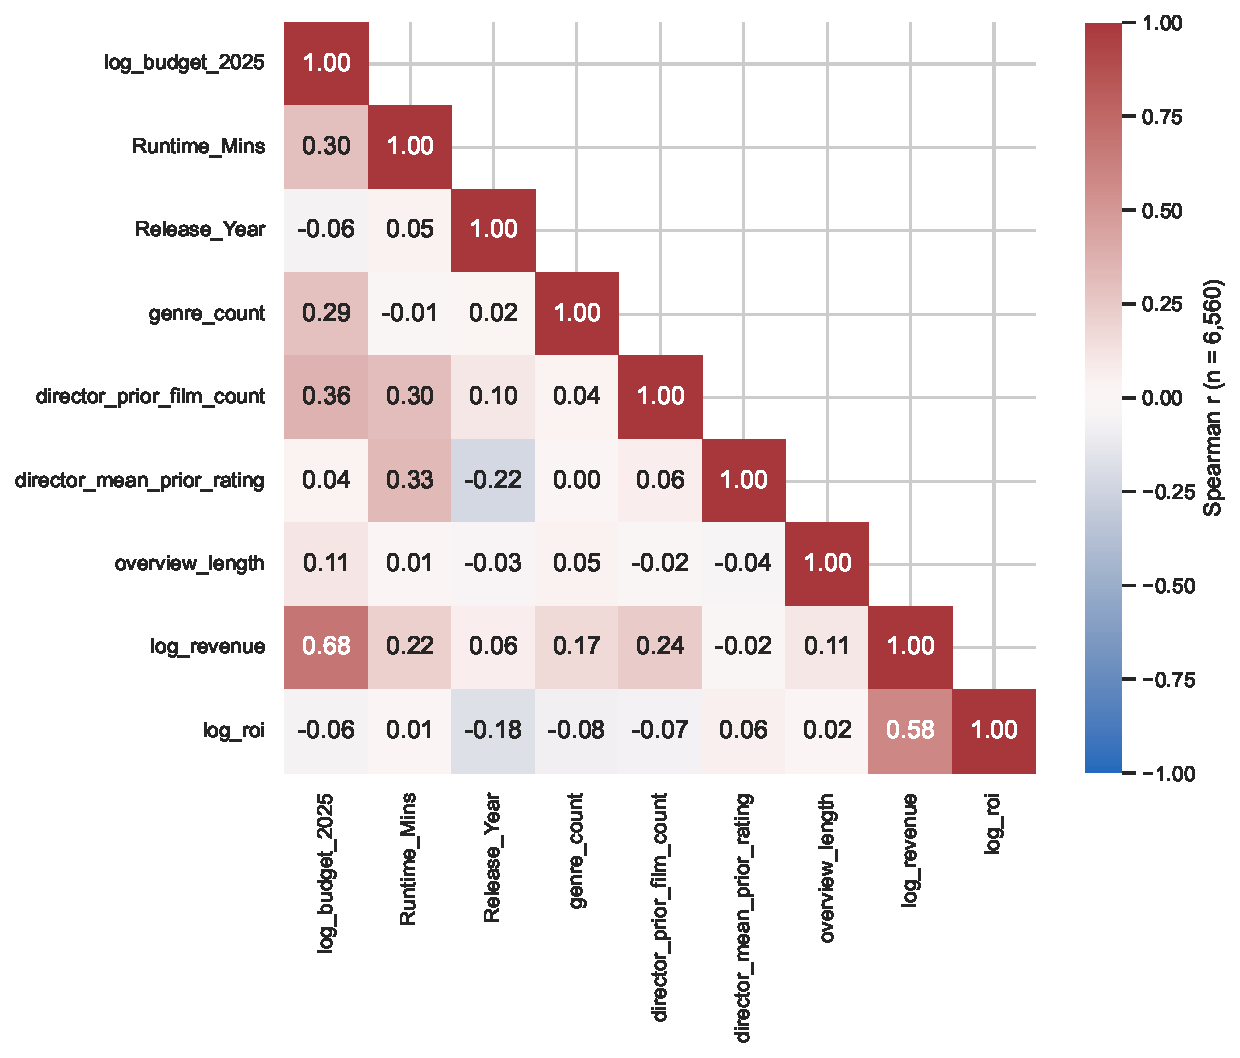
\includegraphics[width=0.85\linewidth]{fig4_1_feature_corr}
\caption{Spearman correlations among the candidate numeric predictors and the two regression targets, $n=\FeatNFinancial$. No pair of predictors comes near the $|r|>0.8$ redundancy threshold. Every predictor correlates far more weakly with log ROI than with log revenue.}
\label{fig:featcorr}
\end{figure}

No pair of candidate predictors exceeds $|r|=0.8$ (Figure~\ref{fig:featcorr}): \FeatCollinearPairsOverZeropEight{} pairs were flagged.

\subsection{Variance inflation factors}

\begin{table}[htbp]
\centering\small
\tablein{tab4_1_vif}
\caption{Variance inflation factors on the standardised numeric block. All are far below the usual concern threshold of 5.}
\label{tab:vif}
\end{table}

Among the real predictors the largest variance inflation factor is \FeatMaxVif{} (Table~\ref{tab:vif}), so the numeric block shows no harmful collinearity. The VIF row for \code{debut\_director} reflects a mechanical link: that indicator marks exactly the films whose prior rating is missing.

\paragraph{A dependency the VIF table cannot see.} \code{genre\_count} is exactly the sum of the one-hot genre flags; the notebook checks this for every film. The two cannot enter a linear model together. A first draft of our OLS model in Chapter~\ref{ch:models} included both. Its genre coefficients were not uniquely determined and shifted by around 3 between runs. We report that mistake because it shows the limit of block-wise VIF checks. \code{genre\_count} is dropped from every model; the more informative genre flags are kept.

\subsection{Mutual information}

\begin{figure}[htbp]
\centering
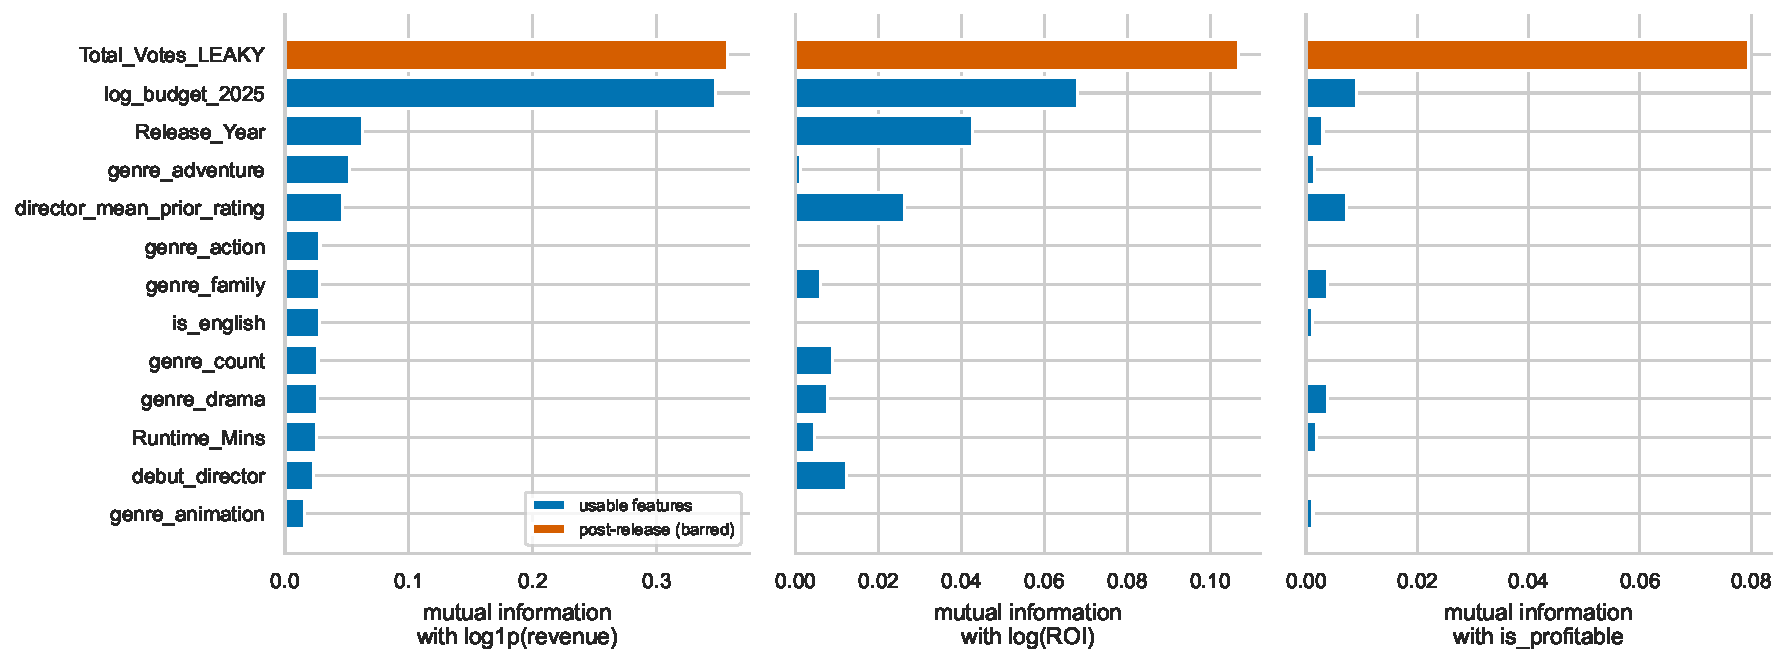
\includegraphics[width=\linewidth]{fig4_2_mutual_info}
\caption{Mutual information between each candidate feature and each of the three targets, $n=\FeatNFinancial$. Budget dominates for revenue. Every feature carries far less information about ROI and profitability than about revenue. The red bar, total votes, is shown only to demonstrate leakage: for profitability it carries several times the information of any legitimate feature.}
\label{fig:mi}
\end{figure}

\begin{table}[htbp]
\centering\small
\tablein{tab4_2_mutual_info}
\caption{Mutual information with each target, top features. ``Total\_Votes (barred)'' is included only to show why post-release data is excluded.}
\label{tab:mi}
\end{table}

Mutual information measures dependence without assuming it is linear (Figure~\ref{fig:mi}, Table~\ref{tab:mi}). Three results shape the next chapter.

\begin{itemize}
  \item \textbf{Budget dominates revenue.} Deflated log budget carries \FeatMiBudgetRevenue{} nats of information about log revenue, far more than any other legitimate feature.
  \item \textbf{ROI is the harder target.} Budget's information about log ROI is \FeatMiBudgetRoi, only \FeatMiRoiToRevenueRatioBudget{} of its information about revenue, and every other feature drops similarly.
  \item \textbf{Post-release data leaks.} If total votes were allowed in, they would match budget on revenue (\FeatMiVotesRevenueLeaky{} against \FeatMiBudgetRevenue). For profitability they would carry \FeatMiLeakRatioProfitable{} times the information of the best legitimate feature (\FeatMiVotesProfitableLeaky{} against \FeatMiBestLegitProfitable). That signal exists only because profitable films go on to collect votes, so votes and popularity are barred.
\end{itemize}

\paragraph{Retained features.} We keep deflated log budget, runtime, the genre flags, English language, the two release-window flags, the director-history pair, studio tier, content rating and overview length. Release year is described but not used as a predictor under the year-based split (Section~\ref{sec:split}). Release quarter and decade duplicate month and year at a coarser resolution, and \code{genre\_count} duplicates the genre flags; all three are dropped.

%%%%%%%%%%%%%%%%%%%%%%%%%%%%%%%%%%%%%%%%%%%%%%%%%%%%%%%%%%%%%%%%%%%%%%%%%%%
\chapter{Model fitting}\label{ch:models}
%%%%%%%%%%%%%%%%%%%%%%%%%%%%%%%%%%%%%%%%%%%%%%%%%%%%%%%%%%%%%%%%%%%%%%%%%%%

In this project, models are tools for measuring which attributes matter and how much of success they can account for; they are not the goal. There are three targets on the \ModelNModel-film financial sample: log revenue in 2025 dollars, log ROI and whether a film is profitable.

\section{Evaluation design}\label{sec:split}

\paragraph{Split by release year, not at random.} A random split would let a model learn from 2019 films and be tested on 2015 films, which is not the situation anyone predicting box office is in. We instead train on films released up to \ModelSplitYear{} ($n=\ModelNTrain$) and test on films released from the year after that through 2025 ($n=\ModelNTest$), the most recent fifth of the data. Release year itself is left out of the predictors, since every test film lies beyond the range of years the model was trained on.

\paragraph{Leakage control.} Imputation, scaling and one-hot encoding all happen inside a scikit-learn \code{Pipeline} \cite{sklearn} that is fitted on the training years only. Votes and popularity are excluded (Chapter~\ref{ch:features}).

\section{Regression}

\subsection{OLS on log revenue}

We first fitted an ordinary least squares (OLS) model with statsmodels \cite{statsmodels}, predicting $\log(1+\text{revenue})$ in 2025 dollars. One genre flag, \code{\ModelOlsDroppedDegenerate}, was dropped because fewer than 10 training films carry it. The model explains $R^2=\ModelOlsRevRTwoTrain$ of the variance on the training years and $R^2=\ModelOlsRevRTwoTest$ on the held-out years.

\paragraph{Diagnostics.} A Breusch--Pagan test rejects constant residual variance ($p=\ModelOlsBpP$) \cite{breusch}, so all standard errors and p-values use the HC3 heteroscedasticity-robust estimator \cite{hc3}. The residuals are left-skewed (skewness \ModelOlsResidSkew): the model's worst misses are films that earned far \emph{less} than their attributes suggest (Figure~\ref{fig:olsdiag}). Flops are less predictable than hits.

\begin{figure}[htbp]
\centering
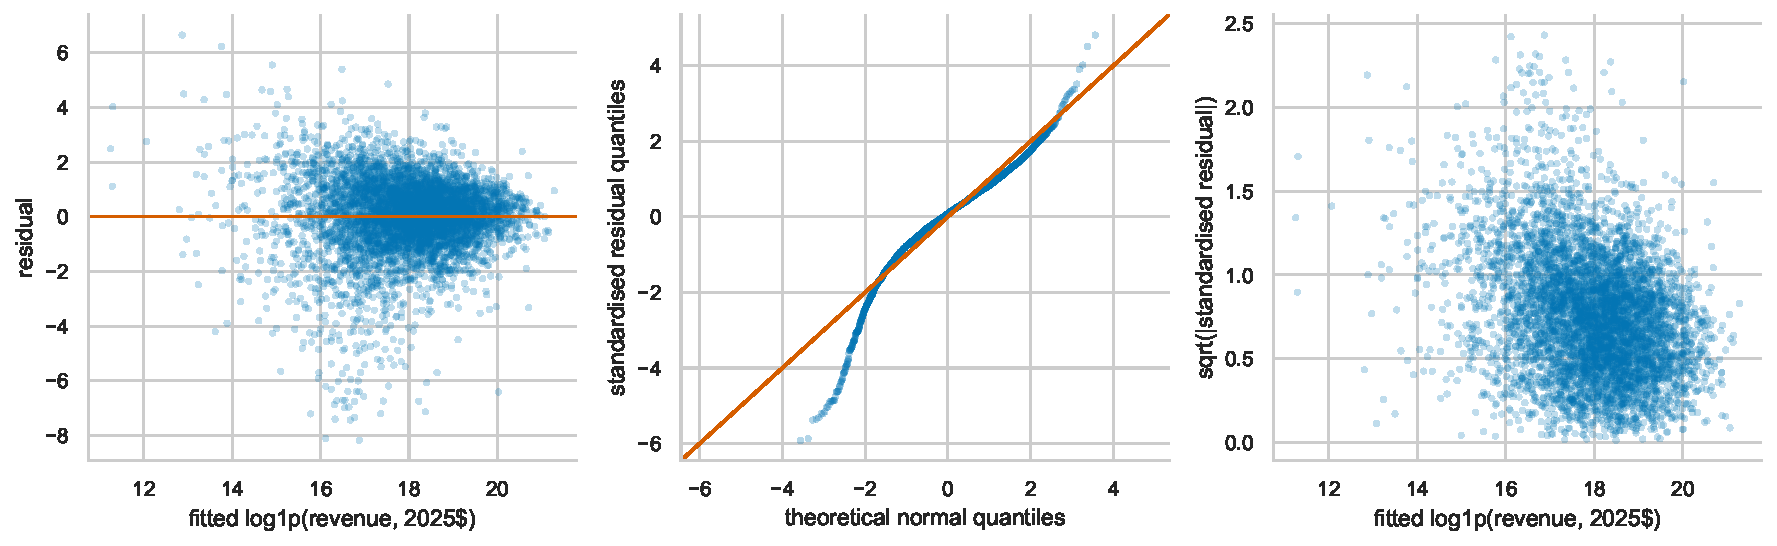
\includegraphics[width=\linewidth]{fig5_1_ols_diagnostics}
\caption{OLS diagnostics on the training years. Left: residuals against fitted values fan out at low fitted revenue. Centre: the Q--Q plot bends away below the line in the left tail, so large shortfalls are more common than a normal distribution allows. Right: the scale--location plot confirms that the spread is not constant. Hence robust (HC3) standard errors throughout.}
\label{fig:olsdiag}
\end{figure}

\begin{table}[htbp]
\centering\small
\tablein{tab5_1_ols_revenue_coefs}
\caption{OLS coefficients on $\log(1+\text{revenue})$, the 15 largest in absolute value, with HC3 robust 95\% intervals and p-values. Log budget enters as a log, so its coefficient is an elasticity; the other coefficients are differences on the log scale, holding the remaining features fixed.}
\label{tab:ols}
\end{table}

Table~\ref{tab:ols} shows the main associations, each holding the other features fixed:

\begin{itemize}
  \item \textbf{Budget.} The coefficient on log budget is \ModelOlsBudgetElasticity{} (95\% CI \ModelOlsBudgetCiLo--\ModelOlsBudgetCiHi, $p=\ModelOlsBudgetP$). A 1\% larger budget is associated with about \ModelOlsBudgetElasticity\% more gross, so gross grows less than proportionally with budget.
  \item \textbf{Studio.} Major-studio films earn more than indie films with otherwise similar attributes (\ModelOlsCoefTierMajor{} on the log scale, $p=\ModelOlsPTierMajor$), and mid-tier studios sit in between (\ModelOlsCoefTierMid).
  \item \textbf{Release window.} Holiday releases (\ModelOlsCoefIsHolidayRelease, $p=\ModelOlsPIsHolidayRelease$) and summer releases (\ModelOlsCoefIsSummerRelease, $p=\ModelOlsPIsSummerRelease$) earn more.
  \item \textbf{Language.} English-language films earn more (\ModelOlsCoefIsEnglish, $p=\ModelOlsPIsEnglish$).
  \item \textbf{Genre.} Documentary (\ModelOlsCoefGenreDocumentary) and Animation (\ModelOlsCoefGenreAnimation) are positive. Drama, Crime and Science Fiction are negative once budget is held fixed. Horror shows no significant difference ($p=\ModelOlsPGenreHorror$).
  \item \textbf{Director.} A director's mean prior rating is weakly positive (\ModelOlsCoefDirectorMeanPriorRating, $p=\ModelOlsPDirectorMeanPriorRating$).
\end{itemize}

\subsection{Regularised and boosted comparisons, and the ROI target}

The same features were fitted with ridge regression, with its penalty chosen by cross-validation within the training years, and with a histogram gradient-boosted tree, which can capture non-linear patterns. All three models were then refitted with log ROI as the target. Table~\ref{tab:reg} and Figure~\ref{fig:predact} compare them.

\begin{table}[htbp]
\centering\small
\resizebox{\linewidth}{!}{\tablein{tab5_2_regression_comparison}}
\caption{Test-set performance on films from \ModelSplitYear{}+1 onwards ($n=\ModelNTest$). Revenue is moderately predictable; ROI almost not at all, by any model.}
\label{tab:reg}
\end{table}

\begin{figure}[htbp]
\centering
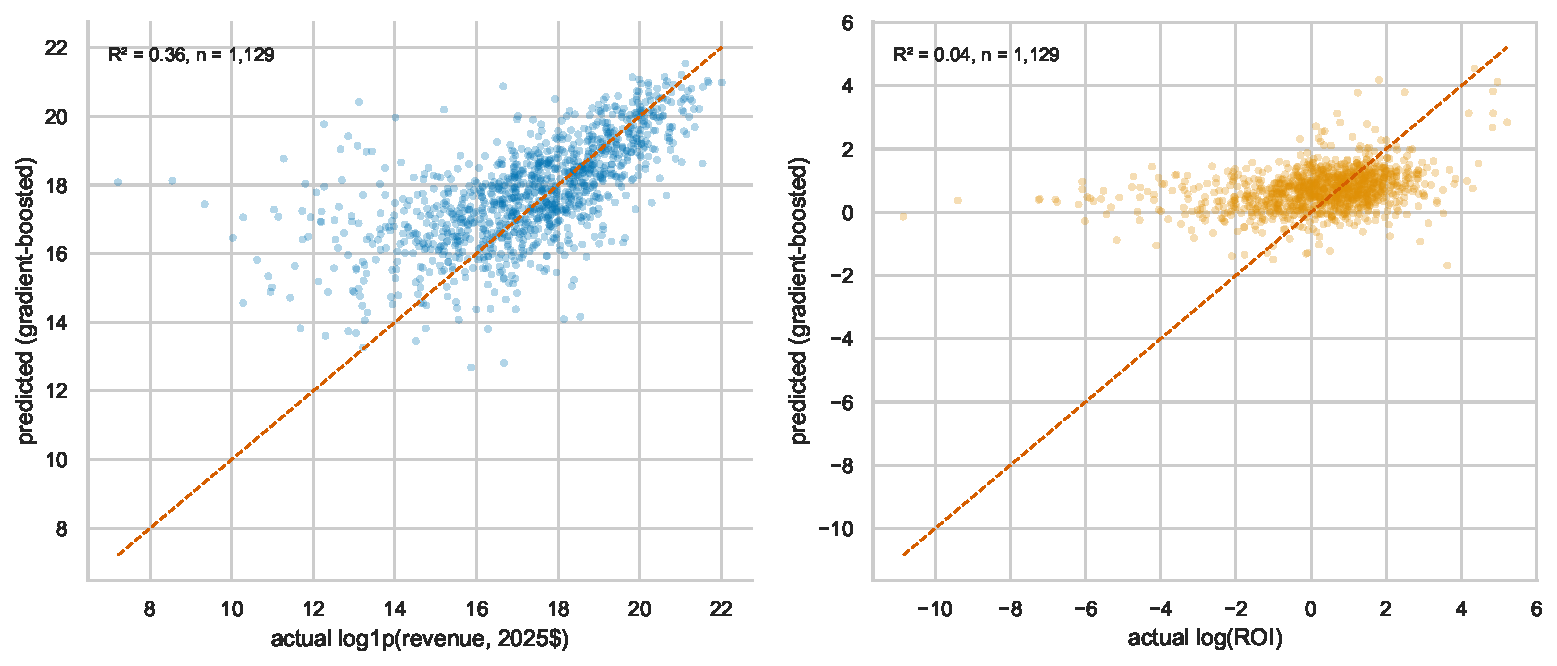
\includegraphics[width=\linewidth]{fig5_2_pred_vs_actual}
\caption{Predicted against actual values on the held-out years (gradient-boosted tree), $n=\ModelNTest$. Revenue predictions follow the diagonal. ROI predictions collapse into a flat band near the average: the model has almost nothing to go on, so it predicts roughly the same return for every film.}
\label{fig:predact}
\end{figure}

\paragraph{The gap between the two targets is the main finding of this chapter.}
\begin{itemize}
  \item \textbf{Revenue is moderately predictable.} Pre-release attributes explain about a third of the variance in log revenue on unseen later years (test $R^2$ from \ModelOlsRevRTwoTest{} to \ModelRidgeRevRTwoTest).
  \item \textbf{ROI is almost unpredictable.} The same attributes explain almost none of the variance in log ROI (test $R^2$ from \ModelOlsRoiRTwoTest{} to \ModelRidgeRoiRTwoTest).
  \item \textbf{No hidden non-linear signal.} The boosted tree does not beat ridge on either target, so the shortfall is not a failure of the linear models to capture complex patterns.
\end{itemize}
What a film \emph{is} (its budget, studio, genre and release slot) largely sets the scale of its gross. How much it returns per dollar depends on things these attributes do not capture: marketing, competition on release weekend, word of mouth and reviews. This pattern matches the long-standing observation that box-office returns are heavy-tailed and hard to forecast \cite{devany}.

\paragraph{Budget and ROI.} With log ROI as the target, the coefficient on log budget is \emph{negative}: \ModelRoiBudgetCoef{} (95\% CI \ModelRoiBudgetCiLo{} to \ModelRoiBudgetCiHi, $p=\ModelRoiBudgetP$). Holding the other attributes fixed, bigger budgets are associated with lower returns per dollar. This agrees with the negative rank correlation in Chapter~\ref{ch:viz}.

\section{Classification}

\paragraph{Target and class balance.} \code{is\_profitable} is true when worldwide gross exceeds production budget. The classes are unbalanced, and the balance shifts over time: \ModelClassBalanceTrain\% of training films are profitable, but only \ModelClassBalanceTest\% of test films. A classifier that always says ``profitable'' would therefore look accurate, so accuracy is not reported. Table~\ref{tab:clf} reports precision, recall, F1 and ROC-AUC, alongside that always-``profitable'' baseline.

\begin{table}[htbp]
\centering\small
\tablein{tab5_3_classification}
\caption{Profitability classification on the held-out years ($n=\ModelNTest$), at a 0.5 probability threshold. F1 barely beats the always-``profitable'' baseline; the AUC shows modest real ability to rank films.}
\label{tab:clf}
\end{table}

\begin{figure}[htbp]
\centering
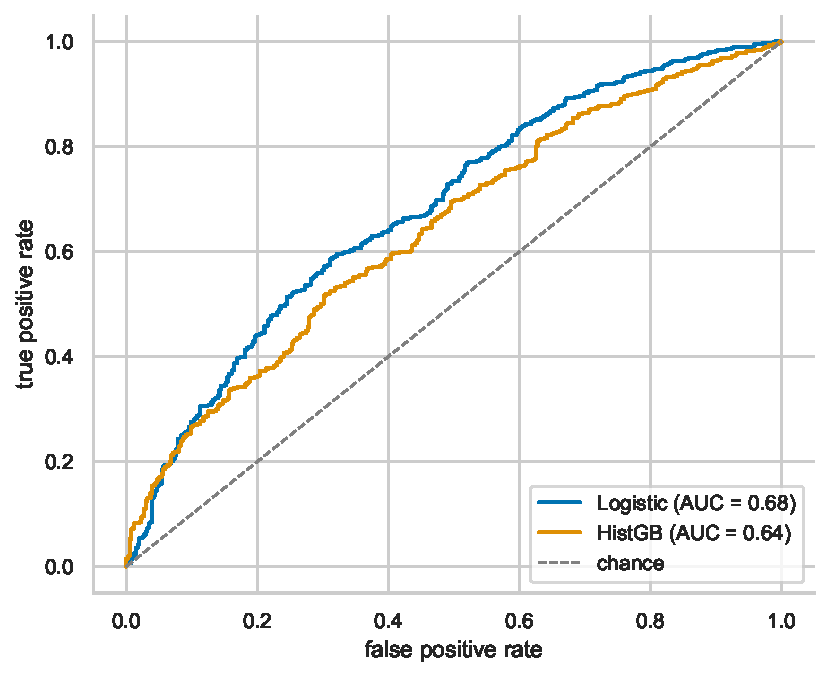
\includegraphics[width=0.6\linewidth]{fig5_3_roc}
\caption{ROC curves on the held-out years. Both classifiers sit clearly above the chance diagonal but far from the top-left corner. Pre-release attributes give a modest head start on profitability, nothing more.}
\label{fig:roc}
\end{figure}

The best F1 score, \ModelClfBestFOne{}, is barely above the baseline's \ModelMajorityBaselineFOne{}. Recall is high and precision modest because, at a 0.5 threshold, the models label nearly every film profitable. The better evidence of skill is the ROC-AUC of \ModelClfBestAuc{} (Figure~\ref{fig:roc}). This is real but modest ranking ability, consistent with the near-zero $R^2$ for log ROI. The drop in the profitable share between the training and test years mirrors the declining ROI of recent decades in Chapter~\ref{ch:viz}.

\section{ML algorithms}

\begin{itemize}
  \item \textbf{Ordinary least squares} (statsmodels). Chosen for interpretability: each coefficient is a conditional association with a confidence interval. Inference uses HC3 robust errors, given the heteroscedasticity found above.
  \item \textbf{Ridge regression} (scikit-learn \code{RidgeCV}). OLS with an L2 penalty that shrinks coefficients and stabilises them when predictors are correlated. The penalty strength was chosen by cross-validation within the training years.
  \item \textbf{Histogram gradient-boosted trees} (scikit-learn). An ensemble of shallow trees that can capture non-linear relationships and interactions. Here it serves as a ceiling check: if it had clearly beaten ridge, the linear summary would be missing structure. It did not.
  \item \textbf{Logistic regression and gradient-boosted classifier} for \code{is\_profitable}.
  \item \textbf{Permutation importance.} How much the boosted revenue model's test $R^2$ falls when one feature's values are randomly shuffled (Figure~\ref{fig:perm}).
\end{itemize}

\begin{figure}[htbp]
\centering
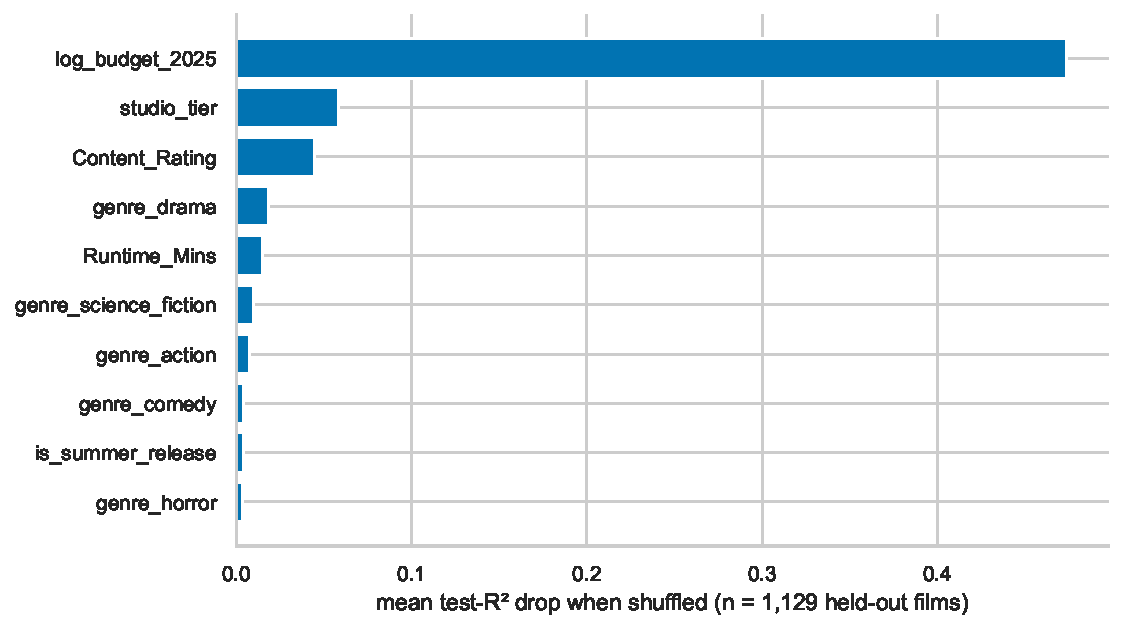
\includegraphics[width=0.8\linewidth]{fig5_4_permutation_importance}
\caption{Permutation importance for the gradient-boosted revenue model on the held-out years: the mean drop in test $R^2$ when each feature is shuffled. Budget towers over everything else; the runner-up is \code{\ModelPermSecondFeature}.}
\label{fig:perm}
\end{figure}

Shuffling budget costs the model \ModelPermTopDrop{} of its test $R^2$. The next most important feature, \ModelPermSecondFeature, costs \ModelPermSecondDrop. The OLS coefficients and the mutual information ranking tell the same story: among the attributes in this data, budget is by far the strongest correlate of gross revenue, and nothing comes close.

%%%%%%%%%%%%%%%%%%%%%%%%%%%%%%%%%%%%%%%%%%%%%%%%%%%%%%%%%%%%%%%%%%%%%%%%%%%
\chapter{Conclusion \& future scope}\label{ch:conclusion}
%%%%%%%%%%%%%%%%%%%%%%%%%%%%%%%%%%%%%%%%%%%%%%%%%%%%%%%%%%%%%%%%%%%%%%%%%%%

\section{Findings/observations}

We answer the questions from Chapter~\ref{ch:intro} in turn. Financial answers refer to the \CleanUsableFinancialSample{} well-documented, released films. All of them describe associations; none is a causal claim.

\paragraph{1. Does a larger budget buy a higher return, or only a higher gross?} \emph{Only a higher gross.} Budget is the strongest correlate of revenue in every analysis. Holding the other attributes fixed, a 1\% larger budget goes with about \ModelOlsBudgetElasticity\% more gross (95\% CI \ModelOlsBudgetCiLo--\ModelOlsBudgetCiHi). Against return on investment, however, budget is \emph{negatively} associated: Spearman $r=\MultiRoiBudgetSpearman$ ($p=\MultiRoiBudgetSpearmanP$, $n=\MultiNFinancial$), and an OLS coefficient on log ROI of \ModelRoiBudgetCoef{} ($p=\ModelRoiBudgetP$). Bigger films gross more but return less per dollar.

\paragraph{2. Which genres give the best rating per dollar?} By the raw ratio, \MultiValueTopGenre{} (\MultiValueTopRatio{} rating points per \$10M of median budget) and \MultiValueSecondGenre{} lead, and \MultiValueBottomGenre{} trails (\MultiValueBottomRatio). The ratio flatters cheap genres, though: horror has the lowest median rating of any genre. The more telling result is that across genres, median budget and median rating show no detectable relationship ($r=\MultiGenreBudgetRatingSpearman$, $p=\MultiGenreBudgetRatingP$, $n=\MultiGenreBudgetRatingN$). \MultiValueTopRatingGenre{} films are the best rated (\MultiValueTopRating) on middling budgets. On commercial return the folklore also fails: \MultiGenreTopMedianRoi{} has the highest median ROI (\MultiGenreTopMedianRoiValue), and horror's famous mean ROI is the product of two outliers.

\paragraph{3. Has mid-budget profitability changed since 2000?} \emph{Not through 2019; sharply since.} Films budgeted at \$20M--\$80M (2025 dollars) had essentially the same median ROI in the 2000s (\MultiMidRoiTwoZeroZeroZeros) and the 2010s (\MultiMidRoiTwoZeroOneZeros; $p=\MultiMidTwoZeroZeroZerosVsTwoZeroOneZerosP$). In 2020--25 the median fell to \MultiMidRoiTwoZeroTwoZeros, and the profitable share dropped from \MultiMidPctProfTwoZeroOneZeros\% to \MultiMidPctProfTwoZeroTwoZeros\% ($p=\MultiMidChiTwoP$). The data cannot separate the pandemic, the shift to streaming and incomplete revenue for recent releases. All three point the same way.

\paragraph{4. Is release timing associated with revenue?} \emph{Yes.} The median \MultiBestMonthName{} release grossed \MultiJuneToSeptemberRatio{} times the median \MultiWorstMonthName{} release (Kruskal--Wallis $p=\MultiMonthKruskalP$). Holding budget, studio and genre fixed, holiday and summer releases still earn more (\ModelOlsCoefIsHolidayRelease{} and \ModelOlsCoefIsSummerRelease{} on the log scale). Studios choose the date, so part of this reflects which films are released when, not the date itself.

\paragraph{5. Do critical and commercial success go together, and can they be predicted?} \emph{Barely, and only the commercial part.} Rating and revenue are almost uncorrelated ($r=\MultiRatingRevenueSpearman$, $n=\MultiNFinancial$). Pre-release attributes explain about a third of the variance in log revenue on unseen later years (test $R^2=\ModelRidgeRevRTwoTest$), but almost none of the variance in log ROI (test $R^2\le\ModelRidgeRoiRTwoTest$). Profitability can be ranked only modestly (ROC-AUC \ModelClfBestAuc). The contrast between a fairly predictable gross and an unpredictable return is, in our view, the most important finding in this project.

\section{Challenges}\label{sec:challenges}

\paragraph{Missing financials that are not missing at random.} The \CleanMarNUndoc{} released films without financials are newer, less voted-on, less popular and less often in English than the documented ones. We chose not to impute, which keeps every financial number honest but limits what those numbers describe: well-documented, mainstream, mostly English-language cinema.

\paragraph{Survivorship.} Every film in the data has at least \AuditTotalVotesMin{} votes. Obscure films, and many outright failures, are simply absent, so the success rates here are higher than those of all films ever made. Survivorship also flatters older decades: an old film is included only if people still rate it today, which favours that era's hits. This bias shapes every conclusion, not only a footnote.

\paragraph{Nominal dollars.} Raw budgets and revenues span 1895--2026 in nominal dollars. We deflated both with the US CPI. That corrects for general inflation, but not for changes in ticket prices relative to other prices, or for exchange rates on non-US revenue.

\paragraph{Marketing spend, the largest omitted variable.} Marketing budgets for major releases are often comparable to production budgets. They rise with production budget, and they are absent from the data. The budget coefficients in this report almost certainly absorb part of marketing's association with revenue. The same omission means our break-even line, revenue equal to production budget, is too lenient: once marketing and the exhibitors' share of ticket sales are counted, fewer films are truly profitable than the \FeatPctProfitable\% this data suggests.

\paragraph{Data quality in the financial columns.} TMDB budgets and revenues are contributed, not audited. \MultiPctBudgetsRoundMillion\% of budgets are exact multiples of \$1M. Streaming originals carry token ``revenue'' that is not comparable to box office. Recent releases may still be accumulating revenue. Each of these adds noise, and the last may exaggerate the recent decline in ROI.

\paragraph{Joining on titles.} The two files share no key, so they were matched on normalised title and year. A title shared by two different films released in the same year could be mismatched. The near-perfect rating agreement suggests such errors are rare.

\section{Future plan}

\begin{itemize}
  \item \textbf{Add marketing and distribution data}, for example advertising spend estimates and opening theatre counts, to test how much of budget's association with revenue is really marketing's.
  \item \textbf{Split revenue into domestic and international}, using sources such as Box Office Mojo, and deflate each with the relevant price index.
  \item \textbf{Measure cast pull without leakage.} Compute each actor's prior box-office record from strictly earlier films, as we did for directors.
  \item \textbf{Treat streaming releases separately.} Identify streaming originals and either exclude them or model them separately, since their ``revenue'' is not box office.
  \item \textbf{Use models suited to heavy tails}, such as quantile regression, to describe what predicts a flop or a breakout rather than only the average film.
  \item \textbf{Use the synopsis text}, for example topic models on \code{Overview}, to capture premise and tone, which genre labels only approximate.
\end{itemize}

%%%%%%%%%%%%%%%%%%%%%%%%%%%%%%%%%%%%%%%%%%%%%%%%%%%%%%%%%%%%%%%%%%%%%%%%%%%
\chapter*{Group Contribution }
\addcontentsline{toc}{chapter}{Group Contribution}
%%%%%%%%%%%%%%%%%%%%%%%%%%%%%%%%%%%%%%%%%%%%%%%%%%%%%%%%%%%%%%%%%%%%%%%%%%%

Work was divided along chapter lines, and the commit history follows the same split. Each member is responsible for the prose of their own chapter; Chapters~5 and~6 are joint.

\section*{Kirtan Kamani (202401094), group leader}
Chapter~1: the research questions, documenting the collection of both datasets and their schemas, and the package list. Repository setup and the shared \code{src/} modules. Assembly and integration of the final report, including the pipeline that generates statistics and tables for it.

\section*{Khanjan Shah (202401092)}
Chapter~2: the data audit, every cleaning rule in \code{clean.py}, the zero-as-missing conversion, the missingness investigation and the decision not to impute, the secondary-dataset join and cross-validation, CPI deflation, and the row reconciliation.

\section*{Shyam Bhuva (202401034)}
Chapter~3: all univariate and multivariate visualisations, the shared plotting style, the genre ROI analysis with its Simpson's-paradox check, the release-month and decade analyses, and the rating-per-dollar and mid-budget analyses.

\section*{Het Bhungaliya (202401033)}
Chapter~4: feature extraction in \code{features.py}, including the leak-free director-history features and their verification, studio tiers and release windows; feature selection by correlation filtering, VIF and mutual information; and identifying the leakage in post-release variables.

\section*{Joint work}
Chapter~5 (model design, the year-based split, OLS diagnostics, regression and classification) and Chapter~6 (answers to the research questions, challenges, future scope).

%%%%%%%%%%%%%%%%%%%%%%%%%%%%%%%%%%%%%%%%%%%%%%%%%%%%%%%%%%%%%%%%%%%%%%%%%%%
\chapter*{Short Bio}
\addcontentsline{toc}{chapter}{Short Bio}
%%%%%%%%%%%%%%%%%%%%%%%%%%%%%%%%%%%%%%%%%%%%%%%%%%%%%%%%%%%%%%%%%%%%%%%%%%%
\begin{multicols}{2}
\textbf{Kirtan Kamani} (202401094) is a BTech student at Dhirubhai Ambani University, Gandhinagar, and led this project group. For this project Kirtan framed the research questions, documented how both datasets were collected, set up the shared code repository and integrated the final report.

\medskip
\textbf{Khanjan Shah} (202401092) is a BTech student at Dhirubhai Ambani University, Gandhinagar. Khanjan led the data-cleaning work for this project: auditing the raw data, treating TMDB's zero-coded financials as missing, testing whether that missingness was random, and deciding against imputation.

\medskip
\textbf{Shyam Bhuva} (202401034) is a BTech student at Dhirubhai Ambani University, Gandhinagar. Shyam led the visualisation work for this project, designing the shared figure style and the univariate and multivariate analyses of budget, revenue, ROI, genre and release timing.

\medskip
\textbf{Het Bhungaliya} (202401033) is a BTech student at Dhirubhai Ambani University, Gandhinagar. Het led the feature-engineering work for this project, building leak-free director-history features and studio tiers and selecting features with correlation, VIF and mutual-information diagnostics.
\end{multicols}

%%%%%%%%%%%%%%%%%%%%%%%%%%%%%%%%%%%%%%%%%%%%%%%%%%%%%%%%%%%%%%%%%%%%%%%%%%%
\chapter*{References}
\addcontentsline{toc}{chapter}{References}
\renewcommand{\chapter}[2]{}
\begin{thebibliography}{99}

\bibitem{tmdb}
The Movie Database (TMDB). \emph{TMDB API documentation.}
\emph{URL:} \url{https://developer.themoviedb.org/docs}

\bibitem{kaggle}
Ahsan Aseer. \emph{Top Rated TMDB Movies 10K} (dataset). Kaggle.
\emph{URL:} \url{https://www.kaggle.com/datasets/ahsanaseer/top-rated-tmdb-movies-10k}

\bibitem{fred}
U.S. Bureau of Labor Statistics. \emph{Consumer Price Index for All Urban Consumers: All Items in U.S. City Average (CPIAUCNS)}, retrieved from FRED, Federal Reserve Bank of St.\ Louis.
\emph{URL:} \url{https://fred.stlouisfed.org/series/CPIAUCNS}

\bibitem{rubin1976}
Rubin, Donald B. \emph{Inference and Missing Data}. \emph{Biometrika}, 63(3), 581--592, 1976.

\bibitem{littlerubin}
Little, Roderick J. A., and Rubin, Donald B. \emph{Statistical Analysis with Missing Data}, 3rd ed. Wiley, 2019.

\bibitem{breusch}
Breusch, Trevor S., and Pagan, Adrian R. \emph{A Simple Test for Heteroscedasticity and Random Coefficient Variation}. \emph{Econometrica}, 47(5), 1287--1294, 1979.

\bibitem{hc3}
MacKinnon, James G., and White, Halbert. \emph{Some Heteroskedasticity-Consistent Covariance Matrix Estimators with Improved Finite Sample Properties}. \emph{Journal of Econometrics}, 29(3), 305--325, 1985.

\bibitem{devany}
De Vany, Arthur, and Walls, W. David. \emph{Uncertainty in the Movie Industry: Does Star Power Reduce the Terror of the Box Office?} \emph{Journal of Cultural Economics}, 23(4), 285--318, 1999.

\bibitem{sklearn}
Pedregosa, Fabian, et al. \emph{Scikit-learn: Machine Learning in Python}. \emph{Journal of Machine Learning Research}, 12, 2825--2830, 2011.

\bibitem{statsmodels}
Seabold, Skipper, and Perktold, Josef. \emph{statsmodels: Econometric and Statistical Modeling with Python}. Proceedings of the 9th Python in Science Conference, 2010.

\bibitem{pandas}
McKinney, Wes. \emph{Data Structures for Statistical Computing in Python}. Proceedings of the 9th Python in Science Conference, 2010.

\bibitem{missingno}
Bilogur, Aleksey. \emph{Missingno: a missing data visualization suite}. \emph{Journal of Open Source Software}, 3(22), 547, 2018.

\end{thebibliography}
\end{document}
